\documentclass[11pt,letterpaper]{article}
\usepackage[utf8x]{inputenc}
\usepackage{float}
\usepackage{quoting}
\usepackage{mdframed}
\usepackage{thm-restate}
\quotingsetup{vskip=0pt,leftmargin=20pt,rightmargin=20pt}

% options for preamble

\def\showauthornotes{0}
\def\showtableofcontents{0} 
\def\showkeys{0}
\def\showdraftbox{0}
\def\showcolorlinks{1}
\def\usemicrotype{1}
\def\showfixme{0}
\def\showdefine{0}

% {{{ etex }}}
\newcommand\hmmax{0}
\newcommand\bmmax{0}
\usepackage{etex}

% {{{ nag }}}

\usepackage[l2tabu, orthodox]{nag}

% {{{ common }}}

\usepackage{xspace,enumerate}

\usepackage[dvipsnames]{xcolor}

\usepackage[T1]{fontenc}
\usepackage[full]{textcomp}

% {{{ babelamerican }}}
\usepackage[american]{babel}

% {{{ mathtools }}}

\usepackage{mathtools}


% {{{ boldmath }}}

% fix for "too many math alphabets" problem
%\newcommand\hmmax{0} % default 3
% \usepackage{bm}

% \usepackage{stmaryrd}


% {{{ amsthm }}}
\usepackage{amsthm}

\newtheorem{theorem}{Theorem}[section]
\newtheorem*{theorem*}{Theorem}
\newtheorem{itheorem}{Theorem}

\newtheorem{subclaim}{Claim}[theorem]
\newtheorem{proposition}[theorem]{Proposition}
\newtheorem*{proposition*}{Proposition}
\newtheorem{lemma}[theorem]{Lemma}
\newtheorem*{lemma*}{Lemma}
\newtheorem{corollary}[theorem]{Corollary}
\newtheorem*{conjecture*}{Conjecture}
\newtheorem{fact}[theorem]{Fact}
\newtheorem*{fact*}{Fact}
\newtheorem{hypothesis}[theorem]{Hypothesis}
\newtheorem*{hypothesis*}{Hypothesis}
\newtheorem{conjecture}[theorem]{Conjecture}


\theoremstyle{definition}
\newtheorem{definition}[theorem]{Definition}
\newtheorem{construction}[theorem]{Construction}
\newtheorem{example}[theorem]{Example}
\newtheorem{question}[theorem]{Question}
\newtheorem{openquestion}[theorem]{Open Question}
\newtheorem{algorithm}[theorem]{Algorithm}
\newtheorem{problem}[theorem]{Problem}
\newtheorem{protocol}[theorem]{Protocol}
\newtheorem{assumption}[theorem]{Assumption}

\theoremstyle{remark}
\newtheorem{claim}[theorem]{Claim}
\newtheorem*{claim*}{Claim}
\newtheorem{remark}[theorem]{Remark}
\newtheorem*{remark*}{Remark}
\newtheorem{observation}[theorem]{Observation}
\newtheorem*{observation*}{Observation}



% {{{ geometry-nice }}}

\usepackage[
letterpaper,
top=0.7in,
bottom=0.9in,
left=1in,
right=1in]{geometry}

% {{{ fonts }}}

%\usepackage{newpxtext} % T1, lining figures in math, osf in text
%\usepackage{textcomp} % required for special glyphs
%\usepackage[varg,bigdelims]{newpxmath}

\usepackage[varg]{pxfonts}
\usepackage{textcomp}
\usepackage[scr=rsfso]{mathalfa}% \mathscr is fancier than \mathcal
\usepackage{bm} % load after all math to give access to bold math
% \useosf %no longer needed
\linespread{1.08}% Give Palatino more leading (space between lines)
\let\mathbb\varmathbb

% {{{ showkeys }}}

\ifnum\showkeys=1
\usepackage[color]{showkeys}
\fi

% {{{ hyperref-option2 }}}

%\ifnum\showcolorlinks=1
\usepackage{hyperref}
\hypersetup{
pagebackref,
% letterpaper=true,
colorlinks=true,
urlcolor=blue,
linkcolor=blue,
citecolor=OliveGreen,
}
\usepackage{prettyref}


\let\pref=\prettyref
%\fi
%
%\ifnum\showcolorlinks=0
%\usepackage[
%pagebackref,
%% letterpaper=true,
%colorlinks=false,
%pdfborder={0 0 0}
%]{hyperref}
%\fi


% {{{ prettyref }}}

% From manual:
% \newrefformat{eq}{\textup{(\ref{#1})}}
% \newrefformat{lem}{Lemma~\ref{#1}}
% \newrefformat{thm}{Theorem~\ref{#1}}
% \newrefformat{cha}{Chapter~\ref{#1}}
% \newrefformat{sec}{Section~\ref{#1}}
% \newrefformat{tab}{Table~\ref{#1} on page~\pageref{#1}}
% \newrefformat{fig}{Figure~\ref{#1} on page~\pageref{#1}}

\newcommand{\savehyperref}[2]{\texorpdfstring{\hyperref[#1]{#2}}{#2}}

\newrefformat{eq}{\savehyperref{#1}{\textup{(\ref*{#1})}}}
\newrefformat{lem}{\savehyperref{#1}{Lemma~\ref*{#1}}}
\newrefformat{def}{\savehyperref{#1}{Definition~\ref*{#1}}}
\newrefformat{thm}{\savehyperref{#1}{Theorem~\ref*{#1}}}
\newrefformat{cor}{\savehyperref{#1}{Corollary~\ref*{#1}}}
\newrefformat{cha}{\savehyperref{#1}{Chapter~\ref*{#1}}}
\newrefformat{sec}{\savehyperref{#1}{Section~\ref*{#1}}}
\newrefformat{app}{\savehyperref{#1}{Appendix~\ref*{#1}}}
\newrefformat{tab}{\savehyperref{#1}{Table~\ref*{#1}}}
\newrefformat{fig}{\savehyperref{#1}{Figure~\ref*{#1}}}
\newrefformat{hyp}{\savehyperref{#1}{Hypothesis~\ref*{#1}}}
\newrefformat{alg}{\savehyperref{#1}{Algorithm~\ref*{#1}}}
\newrefformat{rem}{\savehyperref{#1}{Remark~\ref*{#1}}}
\newrefformat{item}{\savehyperref{#1}{Item~\ref*{#1}}}
\newrefformat{step}{\savehyperref{#1}{step~\ref*{#1}}}
\newrefformat{conj}{\savehyperref{#1}{Conjecture~\ref*{#1}}}
\newrefformat{fact}{\savehyperref{#1}{Fact~\ref*{#1}}}
\newrefformat{prop}{\savehyperref{#1}{Proposition~\ref*{#1}}}
\newrefformat{prob}{\savehyperref{#1}{Problem~\ref*{#1}}}
\newrefformat{claim}{\savehyperref{#1}{Claim~\ref*{#1}}}
\newrefformat{relax}{\savehyperref{#1}{Relaxation~\ref*{#1}}}
\newrefformat{red}{\savehyperref{#1}{Reduction~\ref*{#1}}}
\newrefformat{part}{\savehyperref{#1}{Part~\ref*{#1}}}




% {{{ sref }}}

% short section reference
\newcommand{\Sref}[1]{\hyperref[#1]{\S\ref*{#1}}}

% {{{ nicefrac }}}
% commands for fractions
\usepackage{nicefrac}
% poor man's fraction
\newcommand{\flatfrac}[2]{#1/#2}
\newcommand{\varflatfrac}[2]{#1\textfractionsolidus#2}

\let\nfrac=\nicefrac
\let\ffrac=\flatfrac
% similar commands: tfrac,dfrac

\newcommand{\half}{\nicefrac12}
\newcommand{\onequarter}{\nicefrac14}
\newcommand{\threequarter}{\nicefrac34}

% {{{ microtype-option }}}

\ifnum\usemicrotype=1
\usepackage{microtype}
\fi

% {{{ authornotes }}}
\ifnum\showauthornotes=1
\newcommand{\Authornote}[2]{{\sffamily\small\color{red}{[#1: #2]}}}
\newcommand{\Authornotecolored}[3]{{\sffamily\small\color{#1}{[#2: #3]}}}
\newcommand{\Authorcomment}[2]{{\sffamily\small\color{gray}{[#1: #2]}}}
\newcommand{\Authorstartcomment}[1]{\sffamily\small\color{gray}[#1: }
\newcommand{\Authorendcomment}{]\rmfamily\normalsize\color{black}}
\newcommand{\Authorfnote}[2]{\footnote{\color{red}{#1: #2}}}
\newcommand{\Authorfixme}[1]{\Authornote{#1}{\textbf{??}}}
\newcommand{\Authormarginmark}[1]{\marginpar{\textcolor{red}{\fbox{\Large #1:!}}}}
\else
\newcommand{\Authornote}[2]{}
\newcommand{\Authornotecolored}[3]{}
\newcommand{\Authorcomment}[2]{}
\newcommand{\Authorstartcomment}[1]{}
\newcommand{\Authorendcomment}{}
\newcommand{\Authorfnote}[2]{}
\newcommand{\Authorfixme}[1]{}
\newcommand{\Authormarginmark}[1]{}
\fi

\newcommand{\Dnote}{\Authornote{D}}
\newcommand{\Inote}{\Authornotecolored{ForestGreen}{I}}
\newcommand{\inote}{\Inote}
\newcommand{\Gnote}{\Authornote{G}}
\newcommand{\Jcomment}{\Authorcomment{J}}
\newcommand{\Dcomment}{\Authorcomment{D}}
\newcommand{\Dstartcomment}{\Authorstartcomment{D}}
\newcommand{\Dendcomment}{\Authorendcomment}
\newcommand{\Dfixme}{\Authorfixme{D}}
\newcommand{\Dmarginmark}{\Authormarginmark{D}}
\newcommand{\Dfnote}{\Authorfnote{D}}

%\newcommand{\pnote}{}

\newcommand{\Pfnote}{\Authorfnote{P}}

\newcommand{\PRnote}{\Authornote{PR}}
\newcommand{\PRfnote}{\Authorfnote{PR}}

\newcommand{\RMnote}{\Authornote{RM}}
\newcommand{\RMfnote}{\Authorfnote{RM}}

\newcommand{\PTnote}{\Authornote{PT}}
\newcommand{\PTfnote}{\Authorfnote{PT}}

\newcommand{\PGnote}{\Authornote{PG}}
\newcommand{\PGfnote}{\Authorfnote{PG}}

\newcommand{\Bnote}{\Authornote{B}}
\newcommand{\Bfnote}{\Authorfnote{B}}

\newcommand{\Jnote}{\Authornote{J}}
\newcommand{\Jfnote}{\Authorfnote{J}}


\newcommand{\Mnote}{}
\newcommand{\Mfnote}{\Authorfnote{M}}

\newcommand{\Rnote}{\Authornote{M}}
\newcommand{\Rfnote}{\Authorfnote{M}}

\newcommand{\Nnote}{\Authornote{N}}
\newcommand{\Nfnote}{\Authorfnote{N}}

\newcommand{\Snote}{\Authornote{S}}
\newcommand{\Sfnote}{\Authorfnote{S}}


% {{{ fixme }}}

% place red exclamation mark in margin
%\newcommand{\redmarginmarker}{\marginpar{\textcolor{red}{\fbox{\Large !}}}}
\newcommand{\redmarginmarker}{}

% short indicator for places that need fixing
\newcommand{\FIXME}{\textbf{\textcolor{red}{??}}\redmarginmarker}

\ifnum\showfixme=0
\renewcommand{\FIXME}{}
\fi


% {{{ boxedminipage }}}
\usepackage{boxedminipage}

\newenvironment{mybox}
{\center \noindent\begin{boxedminipage}{1.0\linewidth}}
{\end{boxedminipage}
\noindent
}


% {{{ parentheses }}}
% various bracket-like commands
% round parentheses
\newcommand{\paren}[1]{(#1)}
\newcommand{\Paren}[1]{\left(#1\right)}
\newcommand{\bigparen}[1]{\big(#1\big)}
\newcommand{\Bigparen}[1]{\Big(#1\Big)}
% square brackets
\newcommand{\brac}[1]{[#1]}
\newcommand{\Brac}[1]{\left[#1\right]}
\newcommand{\bigbrac}[1]{\big[#1\big]}
\newcommand{\Bigbrac}[1]{\Big[#1\Big]}
% absolute value
\newcommand{\abs}[1]{\lvert#1\rvert}
\newcommand{\Abs}[1]{\left\lvert#1\right\rvert}
\newcommand{\bigabs}[1]{\big\lvert#1\big\rvert}
\newcommand{\Bigabs}[1]{\Big\lvert#1\Big\rvert}
% cardinality
\newcommand{\card}[1]{\lvert#1\rvert}
\newcommand{\Card}[1]{\left\lvert#1\right\rvert}
\newcommand{\bigcard}[1]{\big\lvert#1\big\rvert}
\newcommand{\Bigcard}[1]{\Big\lvert#1\Big\rvert}
% set
\newcommand{\set}[1]{\{#1\}}
\newcommand{\Set}[1]{\left\{#1\right\}}
\newcommand{\bigset}[1]{\big\{#1\big\}}
\newcommand{\Bigset}[1]{\Big\{#1\Big\}}
% norm
\newcommand{\norm}[1]{\lVert#1\rVert}
\newcommand{\Norm}[1]{\left\lVert#1\right\rVert}
\newcommand{\bignorm}[1]{\big\lVert#1\big\rVert}
\newcommand{\Bignorm}[1]{\Big\lVert#1\Big\rVert}
% 2-norm
\newcommand{\normt}[1]{\norm{#1}_2}
\newcommand{\Normt}[1]{\Norm{#1}_2}
\newcommand{\bignormt}[1]{\bignorm{#1}_2}
\newcommand{\Bignormt}[1]{\Bignorm{#1}_2}
% 2-norm squared
\newcommand{\snormt}[1]{\norm{#1}^2_2}
\newcommand{\Snormt}[1]{\Norm{#1}^2_2}
\newcommand{\bigsnormt}[1]{\bignorm{#1}^2_2}
\newcommand{\Bigsnormt}[1]{\Bignorm{#1}^2_2}
% norm squared
\newcommand{\snorm}[1]{\norm{#1}^2}
\newcommand{\Snorm}[1]{\Norm{#1}^2}
\newcommand{\bigsnorm}[1]{\bignorm{#1}^2}
\newcommand{\Bigsnorm}[1]{\Bignorm{#1}^2}
% 1-norm
\newcommand{\normo}[1]{\norm{#1}_1}
\newcommand{\Normo}[1]{\Norm{#1}_1}
\newcommand{\bignormo}[1]{\bignorm{#1}_1}
\newcommand{\Bignormo}[1]{\Bignorm{#1}_1}
% infty-norm
\newcommand{\normi}[1]{\norm{#1}_\infty}
\newcommand{\Normi}[1]{\Norm{#1}_\infty}
\newcommand{\bignormi}[1]{\bignorm{#1}_\infty}
\newcommand{\Bignormi}[1]{\Bignorm{#1}_\infty}
% inner product
\newcommand{\iprod}[1]{\langle#1\rangle}
\newcommand{\Iprod}[1]{\left\langle#1\right\rangle}
\newcommand{\bigiprod}[1]{\big\langle#1\big\rangle}
\newcommand{\Bigiprod}[1]{\Big\langle#1\Big\rangle}


\newcommand{\ceil}[1]{\lceil #1 \rceil}
% {{{ probability }}}
% expectation, probability, variance
\newcommand{\Esymb}{\mathbb{E}}
\newcommand{\Psymb}{\mathbb{P}}
\newcommand{\Vsymb}{\mathbb{V}}

\DeclareMathOperator*{\E}{\Esymb}
\DeclareMathOperator*{\Var}{\Vsymb}
\DeclareMathOperator*{\ProbOp}{\Psymb}

\renewcommand{\Pr}{\ProbOp}

% TODO: make case distinction if optional argument is not set
\newcommand{\prob}[1]{\Pr\set{#1}}
\newcommand{\Prob}[2][]{\Pr_{{#1}}\Set{#2}}

% \newcommand{\ex}[1]{\E\brac{#1}}
\newcommand{\Ex}[2][]{\E_{{#1}}\Brac{#2}}
\newcommand{\varex}[1]{\E\paren{#1}}
\newcommand{\varEx}[1]{\E\Paren{#1}}

%\newcommand{\given}{\;\middle\vert\;}
\newcommand{\given}{\mathrel{}\middle\vert\mathrel{}}
%\newcommand{\given}{\mathrel{}\middle|\mathrel{}}

% {{{ mathfonts }}}

% \usepackage{dsfont}
% \usepackage{yfonts}
% \usepackage{mathrsfs}


% {{{ miscmacros }}}

% middle delimiter in the definition of a set
\newcommand{\suchthat}{\;\middle\vert\;}

% tensor product
\newcommand{\tensor}{\otimes}

% add explanations to math displays
\newcommand{\where}{\text{where}}
\newcommand{\textparen}[1]{\text{(#1)}}
\newcommand{\using}[1]{\textparen{using #1}}
\newcommand{\smallusing}[1]{\text{(\small using #1)}}
%\ifx\because\undefined
%\newcommand{\because}[1]{\textparen{because #1}}
%\else
%\renewcommand{\because}[1]{\textparen{because #1}}
%\fi
\newcommand{\by}[1]{\textparen{by #1}}


% spectral order (Loewner order)
\newcommand{\sge}{\succeq}
\newcommand{\sle}{\preceq}

% smallest and largest eigenvalue
\newcommand{\lmin}{\lambda_{\min}}
\newcommand{\lmax}{\lambda_{\max}}

\newcommand{\signs}{\set{1,-1}}
\newcommand{\varsigns}{\set{\pm 1}}
\newcommand{\maximize}{\mathop{\textrm{maximize}}}
\newcommand{\minimize}{\mathop{\textrm{minimize}}}
\newcommand{\subjectto}{\mathop{\textrm{subject to}}}

\renewcommand{\ij}{{ij}}

% symmetric difference
\newcommand{\symdiff}{\Delta}
\newcommand{\varsymdiff}{\bigtriangleup}

% set of bits
\newcommand{\bits}{\{0,1\}}
\newcommand{\sbits}{\{\pm1\}}

% no stupid bullets for itemize environmentx
% \renewcommand{\labelitemi}{--}

% control white space of list and display environments
\newcommand{\listoptions}{\labelsep0mm\topsep-0mm\itemindent-6mm\itemsep0mm}
\newcommand{\displayoptions}[1]{\abovedisplayshortskip#1mm\belowdisplayshortskip#1mm\abovedisplayskip#1mm\belowdisplayskip#1mm}

% short for emptyset
%\newcommand{\eset}{\emptyset}
% moved to mathabbreviations

% short for epsilon
%\newcommand{\e}{\epsilon}
% moved to mathabbreviations

% super index with parentheses
\newcommand{\super}[2]{#1^{\paren{#2}}}
\newcommand{\varsuper}[2]{#1^{\scriptscriptstyle\paren{#2}}}

% tensor power notation
\newcommand{\tensorpower}[2]{#1^{\tensor #2}}


% multiplicative inverse
\newcommand{\inv}[1]{{#1^{-1}}}

% dual element
\newcommand{\dual}[1]{{#1^*}}

% subset
%\newcommand{\sse}{\subseteq}
% moved to mathabbreviations

% vertical space in math formula
\newcommand{\vbig}{\vphantom{\bigoplus}}

% setminus
\newcommand{\sm}{\setminus}

% define something by an equation (display)
\newcommand{\defeq}{\stackrel{\mathrm{def}}=}


% define something by an equation (inline)
\newcommand{\seteq}{\mathrel{\mathop:}=}



% declare function f by $f \from X \to Y$
\newcommand{\from}{\colon}

% big middle separator (for conditioning probability spaces)
\newcommand{\bigmid}{~\big|~}
\newcommand{\Bigmid}{~\Big|~}
\newcommand{\Mid}{\;\middle\vert\;}

% better vector definition and some variations
%\renewcommand{\vec}[1]{{\bm{#1}}}
\newcommand{\bvec}[1]{\bar{\vec{#1}}}
\newcommand{\pvec}[1]{\vec{#1}'}
\newcommand{\tvec}[1]{{\tilde{\vec{#1}}}}

% punctuation at the end of a displayed formula
\newcommand{\mper}{\,.}
\newcommand{\mcom}{\,,}

% inner product for matrices
\newcommand\bdot\bullet

% transpose
\newcommand*{\transposed}{\mkern-1mu\intercal}

% indicator function / vector
\ifx\mathds\undefined % use double stroke fonts if available
\newcommand{\Ind}{\mathbb I}
\else
\newcommand{\Ind}{\mathds 1}
\fi

% place a qed symbol inside display formula
%\qedhere

% {{{ superscripts }}}

\renewcommand{\th}{\textsuperscript{th}\xspace}
\newcommand{\st}{\textsuperscript{st}\xspace}
\newcommand{\nd}{\textsuperscript{nd}\xspace}
\newcommand{\rd}{\textsuperscript{rd}\xspace}


% {{{ mathoperators }}}
\DeclareMathOperator{\Inf}{Inf}
\DeclareMathOperator{\Tr}{Tr}
%\newcommand{\Tr}{\mathrm{Tr}}
\DeclareMathOperator{\SDP}{SDP}
\DeclareMathOperator{\sdp}{sdp}
\DeclareMathOperator{\val}{val}
\DeclareMathOperator{\LP}{LP}
\DeclareMathOperator{\OPT}{OPT}
\DeclareMathOperator{\opt}{opt}
\DeclareMathOperator{\vol}{vol}
\DeclareMathOperator{\poly}{poly}
\DeclareMathOperator{\qpoly}{qpoly}
\DeclareMathOperator{\qpolylog}{qpolylog}
\DeclareMathOperator{\qqpoly}{qqpoly}
\DeclareMathOperator{\argmax}{argmax}
\DeclareMathOperator{\polylog}{polylog}
\DeclareMathOperator{\supp}{supp}
\DeclareMathOperator{\dist}{dist}
\DeclareMathOperator{\sign}{sign}
\DeclareMathOperator{\conv}{conv}
\DeclareMathOperator{\Conv}{Conv}

\DeclareMathOperator{\rank}{rank}

% operators with limits
\DeclareMathOperator*{\median}{median}
\DeclareMathOperator*{\Median}{Median}

% smaller summation/product symbols
\DeclareMathOperator*{\varsum}{{\textstyle \sum}}
\DeclareMathOperator{\tsum}{{\textstyle \sum}}

\let\varprod\undefined

\DeclareMathOperator*{\varprod}{{\textstyle \prod}}
\DeclareMathOperator{\tprod}{{\textstyle \prod}}




% {{{ differentials }}}

\newcommand{\diffmacro}[1]{\,\mathrm{d}#1}

\newcommand{\dmu}{\diffmacro{\mu}}
\newcommand{\dgamma}{\diffmacro{\gamma}}
\newcommand{\dlambda}{\diffmacro{\lambda}}
\newcommand{\dx}{\diffmacro{x}}
\newcommand{\dt}{\diffmacro{t}}



% {{{ textabbreviations }}}

% some abbreviations
\newcommand{\ie}{i.e.,\xspace}
%\newcommand{\eg}{e.g.,\xspace}
\newcommand{\Eg}{E.g.,\xspace}
\newcommand{\phd}{Ph.\,D.\xspace}
\newcommand{\msc}{M.\,S.\xspace}
\newcommand{\bsc}{B.\,S.\xspace}

\newcommand{\etal}{et al.\xspace}

\newcommand{\iid}{i.i.d.\xspace}

% {{{ foreignwords }}}

\newcommand\naive{na\"{\i}ve\xspace}
\newcommand\Naive{Na\"{\i}ve\xspace}
\newcommand\naively{na\"{\i}vely\xspace}
\newcommand\Naively{Na\"{\i}vely\xspace}



% {{{ names }}}
% Hungarian/Polish/East European names
\newcommand{\Erdos}{Erd\H{o}s\xspace}
\newcommand{\Renyi}{R\'enyi\xspace}
\newcommand{\Lovasz}{Lov\'asz\xspace}
\newcommand{\Juhasz}{Juh\'asz\xspace}
\newcommand{\Bollobas}{Bollob\'as\xspace}
\newcommand{\Furedi}{F\"uredi\xspace}
\newcommand{\Komlos}{Koml\'os\xspace}
\newcommand{\Luczak}{\L uczak\xspace}
\newcommand{\Kucera}{Ku\v{c}era\xspace}
\newcommand{\Szemeredi}{Szemer\'edi\xspace}
\newcommand{\Hastad}{H{\aa}stad\xspace}
\newcommand{\Hoelder}{H\"{o}lder\xspace}
\newcommand{\Holder}{\Hoelder}
\newcommand{\Brandao}{Brand\~ao\xspace}


% {{{ numbersets }}}
% number sets
\newcommand{\Z}{\mathbb Z}
\newcommand{\N}{\mathbb N}
\newcommand{\R}{\mathbb R}
\newcommand{\C}{\mathbb C}
\newcommand{\Rnn}{\R_+}
\newcommand{\varR}{\Re}
\newcommand{\varRnn}{\varR_+}
\newcommand{\varvarRnn}{\R_{\ge 0}}


% {{{ problems }}}

% macros to denote computational problems

% use texorpdfstring to avoid problems with hyperref (can use problem
% macros also in headings
\newcommand{\problemmacro}[1]{\texorpdfstring{\textup{\textsc{#1}}}{#1}\xspace}

\newcommand{\pnum}[1]{{\footnotesize #1}}

% list of problems
\newcommand{\uniquegames}{\problemmacro{unique games}}
\newcommand{\maxcut}{\problemmacro{max cut}}
\newcommand{\multicut}{\problemmacro{multi cut}}
\newcommand{\vertexcover}{\problemmacro{vertex cover}}
\newcommand{\balancedseparator}{\problemmacro{balanced separator}}
\newcommand{\maxtwosat}{\problemmacro{max \pnum{3}-sat}}
\newcommand{\maxthreesat}{\problemmacro{max \pnum{3}-sat}}
\newcommand{\maxthreelin}{\problemmacro{max \pnum{3}-lin}}
\newcommand{\threesat}{\problemmacro{\pnum{3}-sat}}
\newcommand{\labelcover}{\problemmacro{label cover}}
\newcommand{\setcover}{\problemmacro{set cover}}
\newcommand{\maxksat}{\problemmacro{max $k$-sat}}
\newcommand{\mas}{\problemmacro{maximum acyclic subgraph}}
\newcommand{\kwaycut}{\problemmacro{$k$-way cut}}
\newcommand{\sparsestcut}{\problemmacro{sparsest cut}}
\newcommand{\betweenness}{\problemmacro{betweenness}}
\newcommand{\uniformsparsestcut}{\problemmacro{uniform sparsest cut}}
\newcommand{\grothendieckproblem}{\problemmacro{Grothendieck problem}}
\newcommand{\maxfoursat}{\problemmacro{max \pnum{4}-sat}}
\newcommand{\maxkcsp}{\problemmacro{max $k$-csp}}
\newcommand{\maxdicut}{\problemmacro{max dicut}}
\newcommand{\maxcutgain}{\problemmacro{max cut gain}}
\newcommand{\smallsetexpansion}{\problemmacro{small-set expansion}}
\newcommand{\minbisection}{\problemmacro{min bisection}}
\newcommand{\minimumlineararrangement}{\problemmacro{minimum linear arrangement}}
\newcommand{\maxtwolin}{\problemmacro{max \pnum{2}-lin}}
\newcommand{\gammamaxlin}{\problemmacro{$\Gamma$-max \pnum{2}-lin}}
\newcommand{\basicsdp}{\problemmacro{basic sdp}}
\newcommand{\dgames}{\problemmacro{$d$-to-1 games}}
\newcommand{\maxclique}{\problemmacro{max clique}}
\newcommand{\densestksubgraph}{\problemmacro{densest $k$-subgraph}}


% {{{ alphabet }}}

\newcommand{\cA}{\mathcal A}
\newcommand{\cB}{\mathcal B}
\newcommand{\cC}{\mathcal C}
\newcommand{\cD}{\mathcal D}
\newcommand{\cE}{\mathcal E}
\newcommand{\cF}{\mathcal F}
\newcommand{\cG}{\mathcal G}
\newcommand{\cH}{\mathcal H}
\newcommand{\cI}{\mathcal I}
\newcommand{\cJ}{\mathcal J}
\newcommand{\cK}{\mathcal K}
\newcommand{\cL}{\mathcal L}
\newcommand{\cM}{\mathcal M}
\newcommand{\cN}{\mathcal N}
\newcommand{\cO}{\mathcal O}
\newcommand{\cP}{\mathcal P}
\newcommand{\cQ}{\mathcal Q}
\newcommand{\cR}{\mathcal R}
\newcommand{\cS}{\mathcal S}
\newcommand{\cT}{\mathcal T}
\newcommand{\cU}{\mathcal U}
\newcommand{\cV}{\mathcal V}
\newcommand{\cW}{\mathcal W}
\newcommand{\cX}{\mathcal X}
\newcommand{\cY}{\mathcal Y}
\newcommand{\cZ}{\mathcal Z}

\newcommand{\scrA}{\mathscr A}
\newcommand{\scrB}{\mathscr B}
\newcommand{\scrC}{\mathscr C}
\newcommand{\scrD}{\mathscr D}
\newcommand{\scrE}{\mathscr E}
\newcommand{\scrF}{\mathscr F}
\newcommand{\scrG}{\mathscr G}
\newcommand{\scrH}{\mathscr H}
\newcommand{\scrI}{\mathscr I}
\newcommand{\scrJ}{\mathscr J}
\newcommand{\scrK}{\mathscr K}
\newcommand{\scrL}{\mathscr L}
\newcommand{\scrM}{\mathscr M}
\newcommand{\scrN}{\mathscr N}
\newcommand{\scrO}{\mathscr O}
\newcommand{\scrP}{\mathscr P}
\newcommand{\scrQ}{\mathscr Q}
\newcommand{\scrR}{\mathscr R}
\newcommand{\scrS}{\mathscr S}
\newcommand{\scrT}{\mathscr T}
\newcommand{\scrU}{\mathscr U}
\newcommand{\scrV}{\mathscr V}
\newcommand{\scrW}{\mathscr W}
\newcommand{\scrX}{\mathscr X}
\newcommand{\scrY}{\mathscr Y}
\newcommand{\scrZ}{\mathscr Z}

\newcommand{\bbB}{\mathbb B}
\newcommand{\bbS}{\mathbb S}
\newcommand{\bbR}{\mathbb R}
\newcommand{\bbZ}{\mathbb Z}
\newcommand{\bbI}{\mathbb I}
\newcommand{\bbQ}{\mathbb Q}
\newcommand{\bbP}{\mathbb P}
\newcommand{\bbE}{\mathbb E}
\newcommand{\bbN}{\mathbb N}
\newcommand{\bbD}{\mathbb D}

\newcommand{\sfE}{\mathsf E}


% {{{ leqslant }}}
% slanted lower/greater equal signs
\renewcommand{\leq}{\leqslant}
\renewcommand{\le}{\leqslant}
\renewcommand{\geq}{\geqslant}
\renewcommand{\ge}{\geqslant}


% {{{ draftbox }}}
\ifnum\showdraftbox=1
\newcommand{\draftbox}{\begin{center}
  \fbox{%
    \begin{minipage}{2in}%
      \begin{center}%
%        \begin{Large}%
          \Large\textsc{Working Draft}\\%
%        \end{Large}\\
        Please do not distribute%
      \end{center}%
    \end{minipage}%
  }%
\end{center}
\vspace{0.2cm}}
\else
\newcommand{\draftbox}{}
\fi


% {{{ varepsilon }}}

\let\epsilon=\varepsilon

% {{{ numberequationwithinsection }}}
\numberwithin{equation}{section}


% {{{ restate }}}
% set of macros to deal with restating theorem environments (or anything
% else with a label)

% stolen from Boaz's latex macros

\newcommand\MYcurrentlabel{xxx}

% \MYstore{A}{B} assigns variable A value B
\newcommand{\MYstore}[2]{%
  \global\expandafter \def \csname MYMEMORY #1 \endcsname{#2}%
}

% \MYload{A} outputs value stored for variable A
\newcommand{\MYload}[1]{%
  \csname MYMEMORY #1 \endcsname%
}

% new label command, stores current label in \MYcurrentlabel
\newcommand{\MYnewlabel}[1]{%
  \renewcommand\MYcurrentlabel{#1}%
  \MYoldlabel{#1}%
}

% new label command that doesn't do anything
\newcommand{\MYdummylabel}[1]{}

\newcommand{\torestate}[1]{%
  % overwrite label command
  \let\MYoldlabel\label%
  \let\label\MYnewlabel%
  #1%
  \MYstore{\MYcurrentlabel}{#1}%
  % restore old label command
  \let\label\MYoldlabel%
}

\newcommand{\restatetheorem}[1]{%
  % overwrite label command with dummy
  \let\MYoldlabel\label
  \let\label\MYdummylabel
  \begin{theorem*}[Restatement of \prettyref{#1}]
    \MYload{#1}
  \end{theorem*}
  \let\label\MYoldlabel
}

\newcommand{\restatelemma}[1]{%
  % overwrite label command with dummy
  \let\MYoldlabel\label
  \let\label\MYdummylabel
  \begin{lemma*}[Restatement of \prettyref{#1}]
    \MYload{#1}
  \end{lemma*}
  \let\label\MYoldlabel
}

\newcommand{\restateprop}[1]{%
  % overwrite label command with dummy
  \let\MYoldlabel\label
  \let\label\MYdummylabel
  \begin{proposition*}[Restatement of \prettyref{#1}]
    \MYload{#1}
  \end{proposition*}
  \let\label\MYoldlabel
}

\newcommand{\restatefact}[1]{%
  % overwrite label command with dummy
  \let\MYoldlabel\label
  \let\label\MYdummylabel
  \begin{fact*}[Restatement of \prettyref{#1}]
    \MYload{#1}
  \end{fact*}
  \let\label\MYoldlabel
}

\newcommand{\restate}[1]{%
  % overwrite label command with dummy
  \let\MYoldlabel\label
  \let\label\MYdummylabel
  \MYload{#1}
  \let\label\MYoldlabel
}


% {{{ bibliography }}}

% add section for references to table of contents
\newcommand{\addreferencesection}{
  \phantomsection
  \addcontentsline{toc}{section}{References}
}


% {{{ mathabbreviations }}}

\newcommand{\la}{\leftarrow}
\newcommand{\sse}{\subseteq}
\newcommand{\ra}{\rightarrow}
\newcommand{\e}{\epsilon}
\newcommand{\eps}{\epsilon}
\newcommand{\eset}{\emptyset}


% {{{ paragraphperiod }}}

\let\origparagraph\paragraph
\renewcommand{\paragraph}[1]{\origparagraph{#1.}}
% {{{ allowdisplaybreaks }}}
% allows page breaks in large display math formulas
\allowdisplaybreaks
% {{{ sloppy }}}
% avoid math spilling on margin
\sloppy



% {{{ complexityclasses }}}
\newcommand{\cclassmacro}[1]{\texorpdfstring{\textbf{#1}}{#1}\xspace}
\newcommand{\p}{\cclassmacro{P}}
\newcommand{\np}{\cclassmacro{NP}}
\newcommand{\subexp}{\cclassmacro{SUBEXP}}

% {{{ paralist }}}
\usepackage{paralist}

% {{{ comment }}}
\usepackage{comment}

% {{{ colt hackz }}}
\let\citet\cite
\theoremstyle{definition}




\setcounter{page}{1}

\declaretheorem[name=Proposition,numberwithin=section]{proposition}

%%%%%%%%%%%% Paper specific macros

% paper-specific packages
\usepackage{relsize}
\usepackage[font=footnotesize]{caption}
\usepackage{yfonts}

% abbreviations and paper-specific macros
\newcommand{\Id}{\mathop{\mathrm{Id}}\!\mathinner{}}
\newcommand{\pE}{\tilde {\mathbb E}}
\newcommand{\what}[1]{\widehat{#1}}
\newcommand{\wt}[1]{\widetilde{#1}}
\newcommand{\comp}[1]{\overline{#1}}

\newcommand{\Span}{\mathsf{Span}}
\newcommand{\simp}{\triangle}
\newcommand{\prop}{\textsc{Prop}}

\newcommand*{\annotaterel}[2]{\stackrel{\scriptscriptstyle\text{#1}}{#2}}


\DeclareUrlCommand\email{}


\newcommand{\tnote}[1]{\textcolor{magenta}{\small {\textbf{(Thomas:} #1\textbf{)
      }}}}
\newcommand{\hnote}[1]{\textcolor{blue}{\small {\textbf{(Henry:} #1\textbf{)
      }}}}
      
\usepackage{appendix}
\usepackage{amssymb}
 %\setlength\parindent{0pt}
\usepackage{amsfonts}
\usepackage{latexsym}
\usepackage{amsmath}
\usepackage{qcircuit}
\usepackage{cleveref}


%\usepackage[normalem]{ulem}
%\usepackage{todonotes}
%\newcommand{\hnote}[1]{\todo[inline, color=green!30]{\small{Henry: #1}}}


%%%%%%%%%%%%%%%%%%%%%%%%%%%%%%% QUANTUM MACROS %%%%%%%%%%%%%%%%%

\newcommand{\ket}[1]{|#1\rangle}
\newcommand{\bra}[1]{\langle#1|}
\newcommand{\bigket}[1]{\left |#1 \right \rangle}
\newcommand{\bigbra}[1]{\left \langle#1 \right|}
\newcommand{\ip}[2]{\langle #1 | #2 \rangle}
\newcommand{\ketbra}[2]{|#1\rangle\! \langle #2|}

\newcommand{\Dens}{\mathrm{D}}
\newcommand{\Lin}{\mathrm{L}}


%%%%%%%%%%%%%%%%%%%%%%%%%%%%%%%%%%
\newcommand{\sA}{{\mathsf{A}}}
\newcommand{\sB}{{\mathsf{B}}}
\newcommand{\sC}{{\mathsf{C}}}
\newcommand{\sE}{{\mathsf{E}}}
\newcommand{\sK}{{\mathsf{K}}}
\newcommand{\sM}{{\mathsf{M}}}
\newcommand{\sP}{{\mathsf{P}}}
\newcommand{\sR}{{\mathsf{R}}}
\newcommand{\sS}{{\mathsf{S}}}
\newcommand{\sV}{{\mathsf{V}}}
\newcommand{\sX}{{\mathsf{X}}}
\newcommand{\sY}{{\mathsf{Y}}}
\newcommand{\sZ}{{\mathsf{Z}}}

%\newcommand{\cP}{{\mathcal{P}}}
%\newcommand{\cC}{{\mathcal{C}}}
%\newcommand{\cR}{{\mathcal{R}}}
%\newcommand{\cZ}{{\mathcal{Z}}}
%\newcommand{\cL}{{\mathcal{L}}}

\newcommand{\mS}{\mathcal{S}}

%%%%%%%%%%%%%%%%%%%%%%%%%%%%%%%%%%%

\newcommand{\Hilb}{\mathcal{H}}
\newcommand{\strat}{\mathcal{S}}
\newcommand{\Protocol}{\mathscr{P}}
\newcommand{\reg}[1]{{\textsf{#1}}}
\newcommand{\proj}[1]{\ket{#1}\!\bra{#1}}
\newcommand{\Es}[1]{\textsc{E}_{#1}}
\newcommand{\QMS}{\mathcal{Q}_{\textsc{MS}}}
\newcommand{\MS}{\textsc{MS}}

\newcommand{\NEXPR}{{\sf NEXP}^{(R)}}
\newcommand{\NTIME}{{\sf NTIME}}
\newcommand{\NEXP}{{\sf NEXP}}
\newcommand{\NP}{{\sf NP}}
\newcommand{\MIPstar}{{\sf MIP^*}}

\title{$\MIPstar$ protocols for all $\sf ELEMENTARY$ languages}
\date{}
\author{Joseph Fitzsimons \and Zhengfeng Ji \and Thomas Vidick \and Henry Yuen}


\begin{document}

\maketitle

\section{Introduction}

Ever since the work of Cleve et al.~\cite{cleve2004consequences}, the complexity of computing the value of games with entangled players (known as \emph{entangled games}) has been a central topic of study in quantum complexity theory. Several results in the past several years have provided evidence that this problem is much harder than its classical counterpart. In a breakthrough result, Slofstra showed that there is no algorithm that can decide whether the entangled value of a game is equal to $1$~\cite{slofstra2017set}. Ji showed that estimating the entangled value of a game up to inverse polynomial precision is as hard as solving problems in $\NEXP$ (i.e. nondeterministic exponential time)~\cite{ji2016compression}. In contrast, computing the \emph{classical} value of a game, even approximately, is $\NP$-complete\footnote{More formally, we mean the \emph{decision} version of the problem is $\NP$-complete.}. Since it is known that $\NP$ is a strict subset of $\NEXP$, this shows that the complexity of games is drastically different in the setting of entangled players. 

It is an important open problem to determine both lower and upper bounds on the complexity of approximating the entangled value of a game, as a function of the size of the game and the quality of the approximation.
%A particularly interesting special case of this problem is that of \emph{constant} factor approximation, where given the description of a game $G$, estimate its entangled value $\omega^*(G)$ up to an additive constant $\eps$ that does not depend on $G$. There are two natural conjectures regarding the complexity of this problem. One is that this computational task is complete for $\NEXP$. The other is that this problem is undecidable. There are many other alternative possibilities to these two, but in our view these are the two most reasonable ones. 
%For all we know, the problem of deciding whether the entangled value of a game is $1$ or at most $1/2$ could be undecidable! This question is closely related to deep problems in operator algebras, such as the Connes' Embedding Conjecture~\cite{}. 
The aforementioned results of Slofstra and Ji present lower bounds for exact and inverse exponential approximation factors respectively. Our results in a sense interpolate between these two results. We show a time lower bound on approximating the entangled value of games, where the lower bound scales inversely with the quality of approximation. More precisely, our main result is as follows:

\begin{theorem}
\label{thm:main}
	%Let $R$ be a positive integer. 
	Let $\eps: \N \to (0,1)$ be a monotonically non-increasing function. Any nondeterministic Turing machine $M$ that when given a description of a game $G$ decides whether 
\[
	\omega^*(G) = 1	\qquad \text{or} \qquad \omega^*(G) \leq 1 - \eps(|G|) %\exp(- \underbrace{\exp( \cdots \exp(|G|))}_{R-1})
\]
requires at least $\exp^{(R)}(|G|) := \underbrace{\exp(\exp( \cdots \exp(|G|)))}_{R+1}$ time, where $R$ is any integer such that $\exp^{(R)}(n) = O(1/\eps(n))$ for infinitely many $n \in \N$. Here, $|G|$ refers to the size of the game $G$. \hnote{Make sure number of exponentials is correct.}
\end{theorem}
Roughly speaking, the time complexity of approximating the entangled value of a game $G$ up to accuracy $\eps$ is at least $2^{1/\eps}$ --- even if one were allowed to use nondeterminism. %In fact, we prove a stronger result and show that computing the entangled value up to $\eps$ requires \emph{nondeterministic time} $2^{1/\eps}$\tnote{then why not state the theorem directly this way?}. 


\section{Preliminaries}

For a positive integer quantity $N$ that tends to infinity, and a positive real quantity $\eps$ that tends to zero, we write $\poly[N;\eps]$ to denote a function of the form $N^\alpha \cdot \eps^\beta$ for constants $\alpha, \beta > 0$ that are independent of $N$ and $\eps$.

\paragraph{Iterated exponential}
Let $a,b \in \mathbb{R}$, and let $a > 0$. Let $R \geq 1$ be an integer. We define the iterated exponential function as
\[
	\exp^R_a(b) := 
	\left \{ \begin{array}{ll}
		\exp^{R-1}_a(a^b)	& \mbox{if } b \geq 0 \\
		1/\exp^{R-1}_a(a^{|b|}) & \mbox {if } b < 0
	\end{array}
	\right.
\]
for $R > 1$, and when $R=1$ define $\exp^1_a(b) = a^b$. Equivalently, 
\begin{align*}
	\exp^R_a(b) &:= \underbrace{a^{a^{\cdot^{\cdot^{a^b}}}}}_{R} \qquad \mbox{if } b \geq 0 \\
	\exp^R_a(b) &:= \underbrace{a^{-a^{\cdot^{\cdot^{a^{|b|}}}}}}_{R} \qquad \mbox{if } b < 0
\end{align*}
Furthermore, for convenience we will define $\exp^0_a(b) = b$.% and $\exp^0_a(-b) = 1/b$ when $b \geq 0$.

\subsection{Quantum information theory}

A quantum register is a named finite dimensional Hilbert space. We use san-serif script to denote registers, such as $\sA$, $\sB$, etc. 

Let $\sA$ denote a register.
\begin{enumerate}
	\item $\Dens(\sA)$ denotes the set of density matrices on $\sA$.
	\item $\Lin(\sA)$ denotes the set of linear operators on $\sA$.
\end{enumerate}


\paragraph{State-dependent distance measures}

For a quantum state $\rho \in \Dens(\sA)$ and psd operators $M,N \in \Lin(\sA)$, we define 
\begin{align}
	\Tr_\rho(M) &:= \Tr(M \rho) \\
	\langle M, N \rangle_\rho &:= \Tr_\rho (M^\dagger N) \\
	\Norm{ M }_\rho & := \sqrt{ \langle M, M \rangle_\rho}.
\end{align}

\begin{lemma}
\label{lem:closeness_to_groundspace}
	Let $\sA, \sR$ be registers. Let $H$ be a positive semidefinite matrix acting on $\sA$ with minimum eigenvalue $0$ and second smallest eigenvalue $\Delta > 0$. If $\ket{\psi}$ is a state on $\sA \sR$ such that $\bra{\psi} H_{\sA} \otimes \Id_{\sR} \ket{\psi} \leq \eps$, then there exists a state $\ket{\theta}$ in $\sA \sR$ such that $H \ket{\theta} = 0$ and
	\[
		\left \| \ketbra{\psi}{\psi} - \ketbra{\theta}{\theta} \right \|_1 \leq 4\sqrt{\eps/\Delta}.
	\]
\end{lemma}
\begin{proof}
	Let $P$ denote the projector onto the ground space of $H$ (i.e. the kernel of $H$). Let $Q = \Id - P$. Then since $\Delta Q \preceq H$ we have $\bra{\psi} Q \ket{\psi} \leq \eps/\Delta$. The Gentle Measurement Lemma~\cite{ogawa2002new} states that for all density matrices $\rho$ and for all psd operators $X$ satisfying $0 \preceq X \preceq \Id$, we have
	\[
		\left \| \rho - \sqrt{X}\rho \sqrt{X}  \right \|_1 \leq 2 \sqrt{ \Tr(\rho (\Id - X))}.
	\]
	Setting $\rho = \ketbra{\psi}{\psi}$, $X = P$ and applying the Gentle Measurement Lemma, we obtain the desired conclusion with
	\[
		\ket{\theta} := \frac{ P \ket{\psi}}{\sqrt{ \bra{\psi} P \ket{\psi}}}.
	\]
\end{proof}

\subsection{Quantum interactive protocols} 

We define quantum interactive protocols between a quantum verifier $V$ and provers $P_1,P_2,\ldots,P_r$. In this paper we will focus exclusively on \emph{three-turn protocols}, in which the order of interaction is: the provers send a message to the verifier, the verifier sends a message to the prover, the prover sends a message back, and finally the verifier performs a computation to accept or reject. 

%For simplicity, we will restrict our attention to protocols with a single prover $P$. Extending the discussion to multiple provers is straightforward. 

For simplicity we will first restrict our attention to protocols with a single prover $P$. Our Hilbert space consists of three registers: $\sC, \sV, \sM, \sP$. The verifier $V$ acts on registers $\sC$ (the register containing the prover's initial message), $\sV$ (the verifier's local memory) and $\sM$ (the message register). The prover $P$ acts on $\sM$ and $\sP$ (the prover's local memory). The $\sV$ and $\sM$ registers initially start off in the $\ket{0}$ state, but the $\sC$ and $\sP$ registers are arbitrary (and in general, entangled). The verifier applies a circuit $C_Q$ to $\sC \sV \sM$ ($Q$ stands for ``questions''). The prover then applies some unitary $P$ to $\sM \sP$. The verifier then applies $C_A$ to $\sC \sV \sM$ ($A$ stands for ``answers''). The first output qubit of $\sV$ is measured in the standard basis to determine whether the verifier accepts or rejects.

We can assume without loss of generality that every operation in this protocol is a reflection (Hermitian unitaries that square to identity). The verifier circuits $C_Q,C_A$ consist of Hadamard gates ($H$) and Toffoli gate ($T$), which are reflections. The prover's unitary $P$ can be made a reflection by introducing an ancilla qubit that indicates whether the unitary is to be run forward or backward. In other words, every unitary $P$ can be embedded in a reflection as $\wt{P} = \ketbra{1}{0} \otimes P + \ketbra{0}{1} \otimes P^\dagger$. 

The extension to $r$ provers is straightforward: the registers $\sM$ and $\sP$ are divided into $r$ parts: $\sM_1,\ldots,\sM_r$ and $\sP_1,\ldots,\sP_r$. The $i$-th prover's unitary $P_i$ acts on $\sM_i \sP_i$. 

Pictorially, the protocol looks like Figure \ref{fig:qip}.

\begin{figure}[H]
\begin{center}
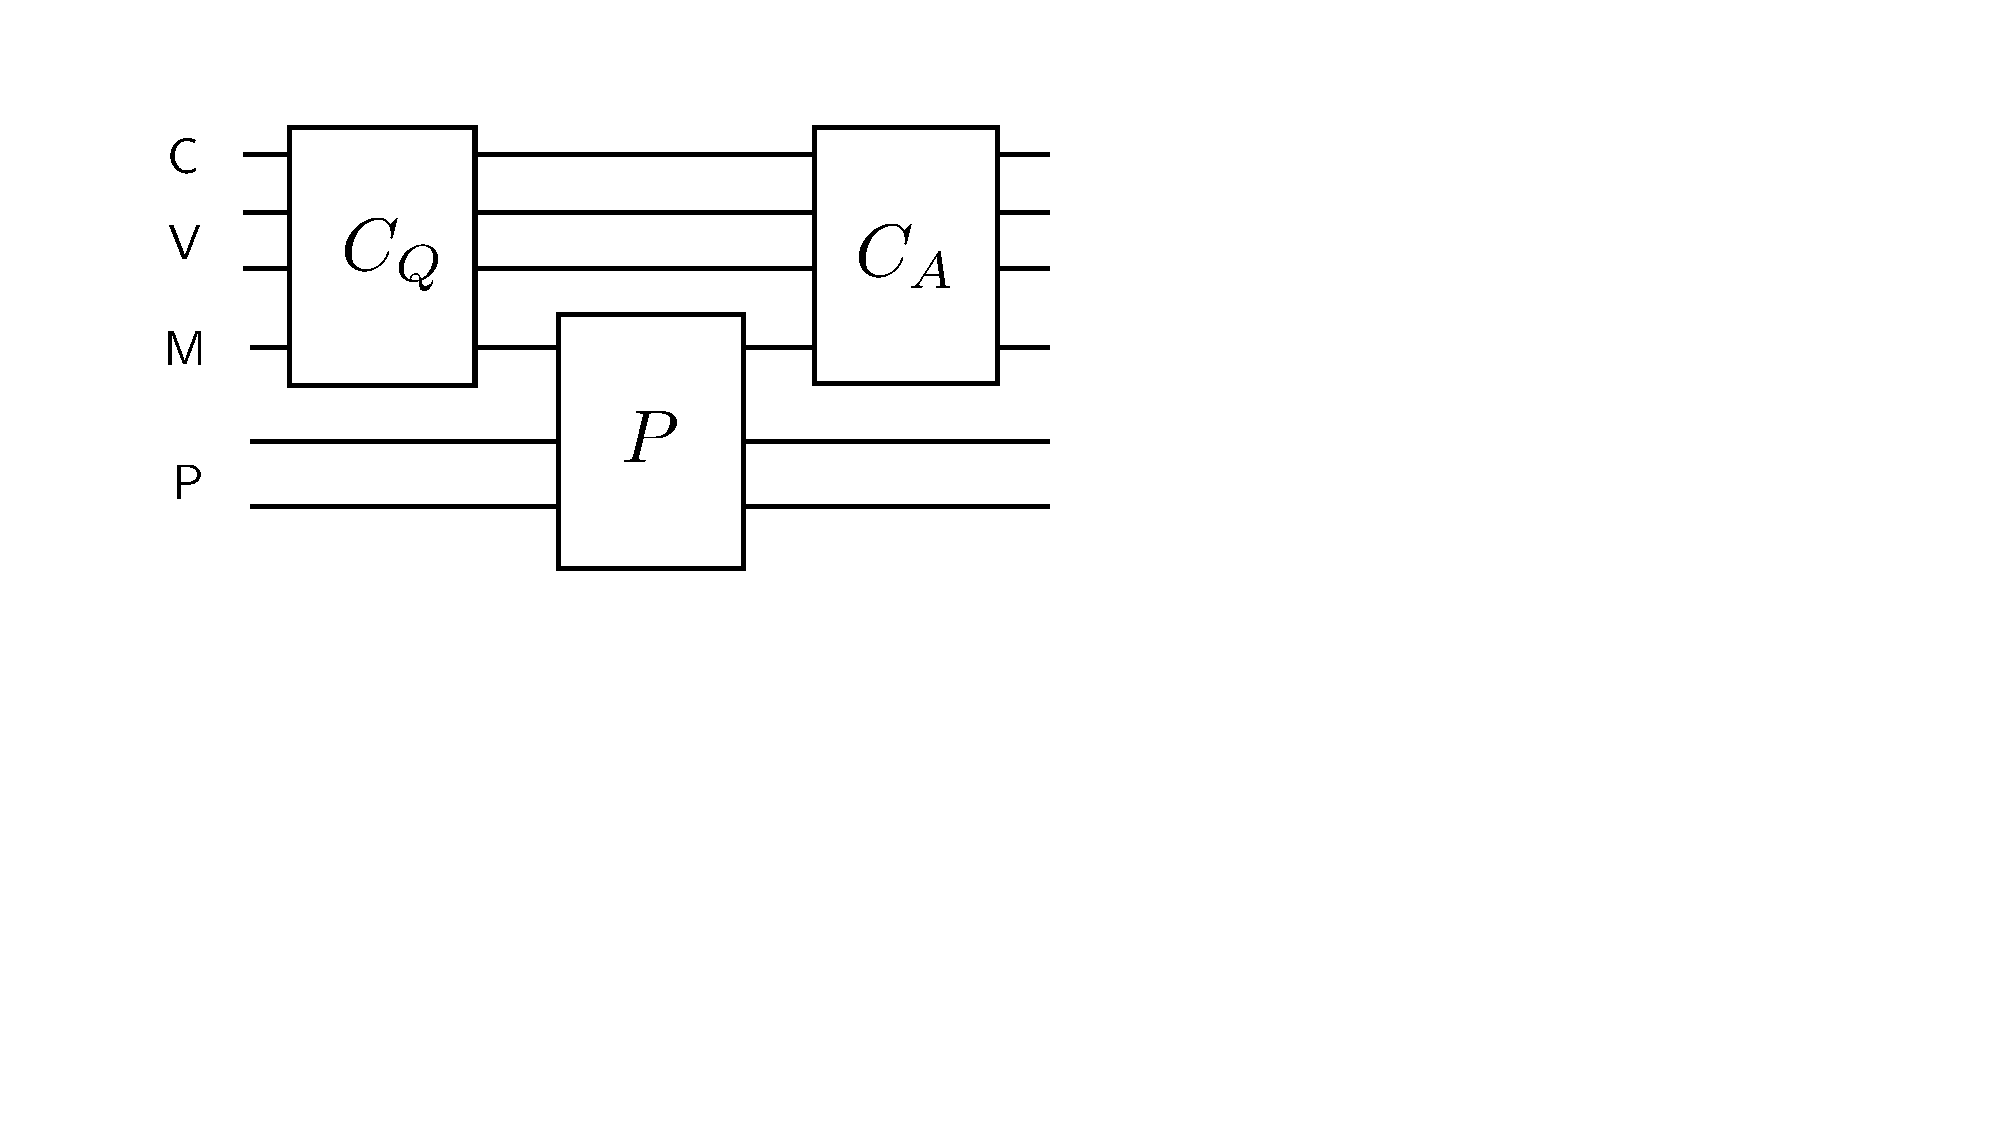
\includegraphics[width=4in]{graphics/qip3.pdf}
\end{center}
\caption{Three-turn quantum interactive protocol.}
\label{fig:qip}
\end{figure}

A verifier $V = (C_Q,C_A)$ will implicitly define $3$-turn quantum interactive protocol for some number of provers. We will let $\Protocol_V$ denote this protocol.

\subsubsection{Strategies}

Let $V = (C_Q,C_A)$ be a verifier for an $r$-prover protocol $\Protocol_V$. A \textbf{strategy} $\strat$ for $\Protocol_V$ consists of a pair $(\rho,\{P_i\})$ where
\begin{enumerate}
	\item $\rho$ is an entangled state on $r+1$ (finite dimensional) registers $\sC, \sP_1, \ldots, \sP_r$
	\item For each $i$, $P_i$ is a reflection acting on the $\sM_i \sP_i$ registers.
\end{enumerate}
Note that given $V$, the size of register $\sC$ is fixed (because it is specified by the verifier circuit $V$) in any strategy $\strat$ for $\Protocol_V$. However, the size of the registers $\paren{ \sP_i}$ can be arbitrary.

The \textbf{value of $\strat$ in $\Protocol_V$} is denoted by $\omega^*_\strat(V)$ and is defined as
\[
	\omega^*_{\strat}(V) := \Tr \Paren{ \Pi_{out} \, \paren{ C_A P C_Q} \, \rho \otimes \ketbra{0}{0}_{\sV \sM} \, \paren{C_A P C_Q}^\dagger}
\]
where $\Pi_{out} = \ketbra{1}{1}_{\sV_{out}}$ is the projector onto the $\ket{1}$ state of the output qubit of the $\sV$ register, $\ketbra{0}{0}_{\sV \sM}$ is the all zeroes state in the $\sV \sM$ registers, and $P = P_1 \otimes \cdots \otimes P_r$. 


The \textbf{value of a protocol $\Protocol_V$} is denoted by $\omega^*(V)$ and is defined as 
\[
	\omega^*(V) := \sup_{\strat} \omega^*_\strat(V)
\]
where the supremum is over all (finite dimensional) strategies $\strat$ for $\Protocol_V$. 

%We can now describe the execution of this interactive protocol as a sequence of gates $G_1,G_2,\ldots,G_\tau$ corresponding to the sequence of Hadamard and Toffoli gates of the verifier circuits interleaved with the prover's unitaries $W_i$. In other words, the gate sequence $\{G_t\}$ consists entirely of Hadamard and Toffoli gates except for the prover's unitaries. %Note that $\tau = \poly(n)$ since the interactive protocol runs in polynomial time.


\subsubsection{Closeness of strategies} 

We now define notions of closeness of strategies. 
%
%\begin{definition}[State-dependent closeness of POVMs]
%	Let $\rho \in \Dens(\sA)$ be a state and let $M = \{M^a\}_a,N = \{N^a\}_a$ be two POVMs that have the same set of possible outcomes. Then define 
%	\begin{align}
%		d_\rho \Paren{ M, N } := \Brac{ \sum_a \Norm{ M^a - N^a }_\rho^2 }^{1/2}.
%	\end{align}
%\end{definition}

\begin{definition}[Closeness of strategies]
	Let $V = (C_Q,C_A)$ be a verifier and let $\strat = (\rho,\{P_i\}), \strat' = (\rho',\paren{P_i'})$ be strategies for the $r$-prover protocol $\Protocol_V$. Then $\strat$ is \textbf{$\eps$-close} to $\strat'$ if and only if
	\begin{enumerate}
		\item $ \norm{ \rho - \rho'}_{tr} \leq \eps$
		\item $\Norm{ P \sigma P^\dagger - P' \sigma P'^\dagger }_{tr} \leq \eps$		
		%For all $i\in\{1,\ldots,r\}$, %for all $q \in \mathcal{Q}_i$,
		%\tnote{why this? the first condition says that having the second for $\rho$ or $\rho'$ is enough}
		
		%d_\rho(M_i(q),M_i'(q)) \leq \eps.
		%\Norm{ P - P' }^2_{\wt{\rho}} \leq \eps
		%\]
	\end{enumerate}
where $\sigma := C_Q \rho \otimes \ketbra{0}{0}_{\sV \sM} C_Q^\dagger$, $P = P_1 \otimes \cdots \otimes P_r$ and $P' = P_1' \otimes \cdots \otimes P_r'$.

\end{definition}

\begin{definition}[Isometric strategies]
	Let $\strat = (\rho,\{P_i\})$ and $\strat' = (\rho',\{P_i'\})$ be strategies for an $r$-prover protocol $\Protocol_V$ corresponding to some verifier $V = (C_Q,C_A)$. Suppose $\rho \in \Dens(\sC \sP_1 \cdots \sP_r)$ and $\rho' \in \Dens(\sC \sP_1' \cdots \sP_r')$. Then $\strat$ is \textbf{$\eps$-isometric} to $\strat'$ if and only if there exist isometries: $I_i : \sP_i \to \sP_i'$ for each $i\in\{1,\ldots,r\}$ such that the strategy $\wt{\strat} = (\wt{\rho}, \set{ \wt{P}_i })$ is $\eps$-close to $\strat'$, where $\wt{\strat}$ is defined by
	\begin{enumerate}
		\item $\wt{\rho} = (I_1 \otimes \cdots \otimes I_r) \rho (I_1 \otimes \cdots \otimes I_r)^\dagger$
		\item For all $i$, $\wt{P}_i = I_i P_i I_i^\dagger$.
	\end{enumerate}
\end{definition}


\begin{lemma}
\label{lem:close_strategies}
	Let $V = (C_Q,C_A)$ be a verifier and let $\strat_1 = (\rho_1,\{P^{(1)}_i\}),\strat_2= (\rho_2,\{P^{(2)}_i\})$ be strategies for $\Protocol_V$ such that $\strat_1$ is $\eps$-isometric to $\strat_2$. Then we have that
	\[
		\Abs{ \omega_{\strat_1}(V) - \omega_{\strat_2}(V) } \leq 2\eps.
	\]
\end{lemma}
\begin{proof}
For notational convenience we omit the all zeroes state $\ketbra{0}{0}_{\sV \sM}$ in the calculations below. Let $\strat_3= (\rho_3,\{P^{(3)}_i\})$ be the strategy such that $\strat_1$ is perfectly isometric to $\strat_3$ and $\strat_3$ is $\eps$-close to $\strat_2$. It is straightforward to verify that $\omega_{\strat_1}(V) = \omega_{\strat_3}(V)$. 
	
	Let $\strat_4 = (\rho_4,\set{ P^{(4)}_i})$ be such that $\rho_4 = \rho_2$ but $\set{P^{(4)}_i} = \set{P^{(3)}_i}$. Then
	\begin{align*}
		\abs{ \omega^*_{\strat_3}(V) - \omega^*_{\strat_4}(V)} &\leq \Abs{ \Tr\Paren{ (C_A P^{(3)} C_Q)^\dagger \Pi_{out} (C_A P^{(3)} C_Q) \paren{\rho_3 - \rho_2}} } \\
		&\leq \norm{ \rho_3 - \rho_2}_{tr} \\
		&\leq \eps.
	\end{align*}
	where $P^{(3)} = \bigotimes P^{(3)}_i$. The second inequality follows from matrix H\"{o}lder ($\Tr(AB) \leq \|A\|_\infty \|B\|_{tr}$) and the last inequality follows from the fact that $\strat_3$ is $\eps$-close to $\strat_2$.
	Next, we have
	\begin{align*}
		\abs{ \omega^*_{\strat_2}(V) - \omega^*_{\strat_4}(V)} &\leq \Abs{ \Tr\Paren{ \Pi_{out} \Paren{ (C_A P^{(2)} C_Q)\rho_2 (C_A P^{(2)} C_Q)^\dagger  - (C_A P^{(3)} C_Q) \rho_2 (C_A P^{(3)} C_Q)^\dagger  } }} \\
		&\leq \norm{ (P^{(2)} C_Q) \rho_2 (P^{(2)} C_Q)^\dagger - (P^{(3)} C_Q) \rho_2 (P^{(3)} C_Q)^\dagger}_{tr} \\
		&\leq \eps.
	\end{align*}	
	The first inequality follows from matrix H\"{o}lder and the second inequality follows again from the fact that $\strat_3$ is $\eps$-close to $\strat_2$. Putting everything together we obtain the desired conclusion.

\end{proof}



\section{Special types of quantum interactive protocols}

In this section we will define a few special types of three-turn quantum interactive protocols that are central to our results. 

%\subsubsection{Non-local games} 

%
%\subsection{Games and strategies}
%
\subsection{Non-local games} 
An $r$-player \textbf{non-local game} $G$ is a tuple $(\mathcal{Q},\mathcal{A},\mu,V)$ where $\mathcal{Q} = \mathcal{Q}_1 \times \cdots \times \mathcal{Q}_r$ and $\mathcal{A} = \mathcal{A}_1 \times \cdots \times \mathcal{A}_r$ are $r$-partite alphabets, $\mu$ is a distribution over $\mathcal{Q}$, and $V: \mathcal{Q} \times \mathcal{A} \to \{0,1\}$ is a verification predicate. 

%A non-local game is played in the following manner. Before the game starts, the players distribute a shared state $\rho_{\sP_1 \cdots \sP_r}$ between themselves where player $i$ gets register $\sP_i$. In the game, the referee uses private randomness to sample a tuple of \emph{questions} $\vec{q} = (q_1,\ldots,q_r)$ from $\mu$, and sends $q_i$ to player $i$, who then performs local measurements on register $\sP_i$ of $\rho$ and returns the measurement outcome $a_i \in \mathcal{A}_i$ (called an \emph{answer}) to the referee. The referee accepts if and only if $V(\vec{q},\vec{a}) = 1$, where $\vec{a} = (a_1,\ldots,a_r)$.

An $r$-player non-local game is a type of three-turn quantum interactive protocol where the circuit $C_Q$ samples questions $\vec{q} = (q_1,\ldots,q_r)$ from the distribution $\mu$, and saves a copy of $q_i$ in the register $\sM_i$. After the provers' unitaries $P = P_1 \otimes \cdots \otimes P_r$, the circuit $C_A$ reads the $\sM$ registers in the standard basis to obtain the answers $\vec{a} = (a_1,\ldots,a_r)$, and then computes the predicate $V(\vec{q},\vec{a})$ to decide whether to accept or reject.


\subsection{Simulated Communication Games}

Here we will define a variant of three-turn protocols, called \textbf{simulated communication games} (or \textbf{SimCom games} for short), where the verifier and provers do not explicitly exchange message registers. Instead, they will use quantum teleportation to communicate. Furthermore, whereas in teleportation the sender transmits classical teleportation keys to the receiver, in SimCom games no such transmission takes place. Instead, the communicating parties will \emph{guess} what the correct teleportation keys are, and we will measure the acceptance probability of the verifier \emph{conditioned} on the event that every party correctly guesses the teleportation keys. This explains why we call the communication \emph{simulated}. 

The benefit of using SimCom games is that the actions of the verifier and the provers are disjoint: they act on separate registers. This will be very useful for us in our recursive compression result. There will be a quantitative loss in transforming normal quantum interactive protocols to SimCom games, but this loss will small provided that the original message lengths were small. 

More precisely, an $r$-prover SimCom game is specified by a verifier $V$, which 
%an $r$-partite question alphabet $\cQ = \cQ_1 \times \cdots \times \cQ_r$, and an $r$-partite answer alphabet $\cA = \cA_1 \times \cdots \times \cA_r$. 
is still specified by two circuits $(C_Q,C_V)$ acting on registers $\sC \sV \sM$. %The $\sM$ register is isomorphic to whichever is the larger of $\cQ$ or $\cA$.\footnote{Here, we abuse notation and treat $\cQ$ (resp. $\cA$) as a Hilbert space of dimension $|\cQ|$ (resp. $|\cA|$).}

However, instead of letting the provers act on $\sM \sP$ as before, the protocol behaves as follows: there are five additional registers $\sE_{1} \sE_{1}' \sE_{2} \sE_{2}' \sK$. The $\sE_j$ and $\sE_j'$ registers are each isomorphic to $\sM$. The $\sK$ register is isomorphic to two copies of $\sM$. The $\sE_1 \sE_1' \sE_2 \sE_2'$ registers are initialized in the state $\ket{\Phi}_{\sE_{1} \sE_{1}'} \otimes \ket{\Phi}_{\sE_{2} \sE_{2}'}$, where $\ket{\Phi}_{\sE_j \sE_j'}$ denotes the maximally entangled state between $\sE_j$ and $\sE_j'$. The $\sK$ register is initialized to all zeroes.

The maximally entangled state $\ket{\Phi}_{\sE_1 \sE_1'}$ will be used to teleport the verifier's outgoing message to the provers; after the circuit $C_Q$, there will be a teleportation circuit $TP$ acting on $\sV \sM \sE_1$, which performs a Bell measurement on $\sM \sE_1$ and stores the measurement outcome in $\sV$. The provers then act on $\sE_1' \sE_2' \sP \sK$, where the $i$-th prover acts on $\sE_{1,i}' \sE_{2,i}' \sP_i \sK_i$. 

Then, a SWAP gate is applied between $\sE_2$ and $\sM$. Finally, the circuit $C_A$ is applied to $\sC \sV \sM$. In addition to the output qubit $\sV_{out}$, we identify additional sub-registers of $\sV$, denoted by $\sV_{tp1},\sV_{tp2}$. These two registers are each isomorphic to two copies of $\sM$.

%The first register $\sV_{tp1}$ is isomorphic to two copies of $\cM$. The second register $\sV_{tp2}$ is isomorphic to two copies of $\cA$. 

See Figure \ref{fig:simcom} for a pictorial representation of a SimCom game.


\begin{figure}[H]
\begin{center}
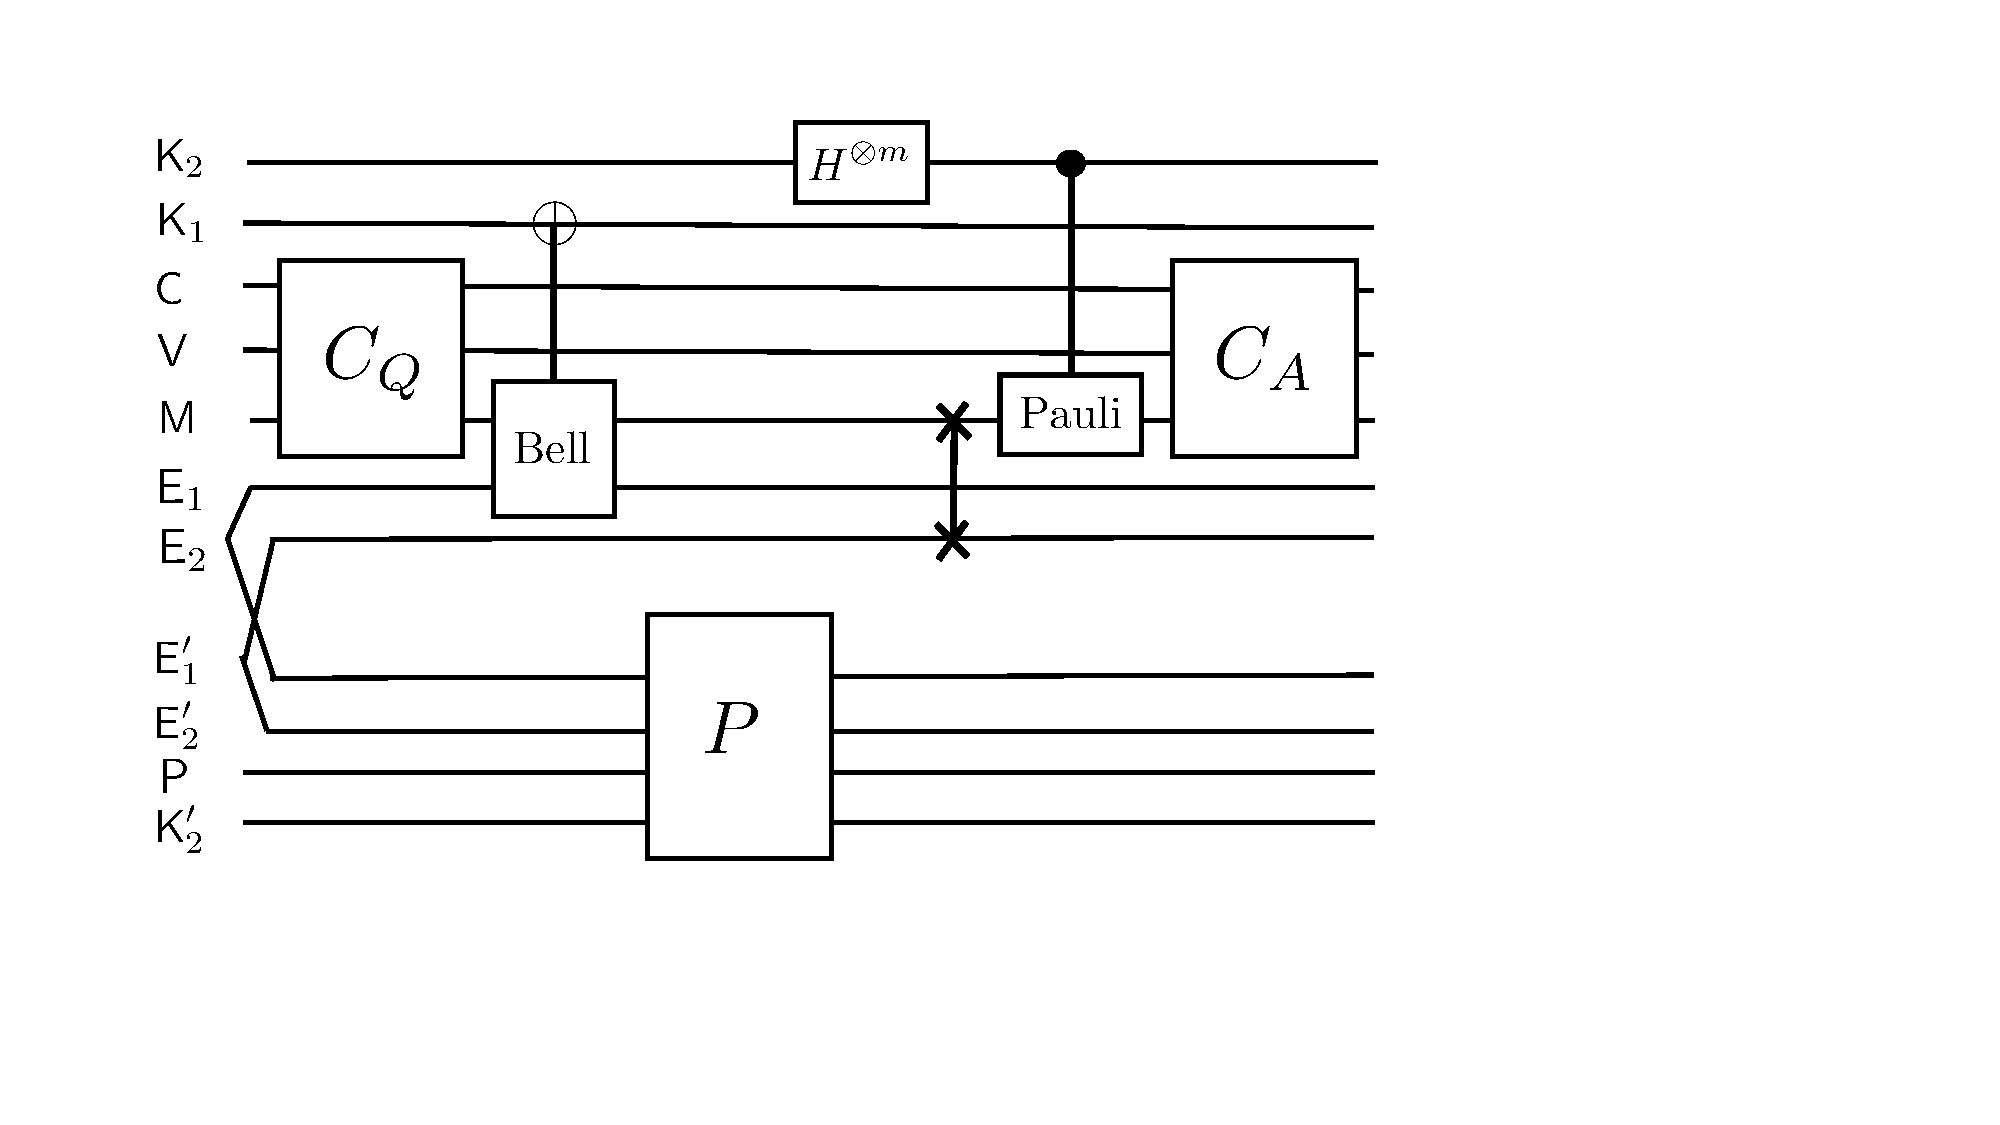
\includegraphics[width=5in]{graphics/simcom.pdf}
\end{center}
\caption{A simulated communication game.}
\label{fig:simcom}
\end{figure}

Let $V = (C_Q,C_A)$ be a verifier and let $\mathscr{Z}_V$ denote the SimCom game corresponding to $V$. We say that $V$ accepts in $\mathscr{Z}_V$ if measuring the $\sV_{out} \sV_{tp1} \sV_{tp2} \sK$ registers yields outcome $(b,t_1,t_2,k)$ where $b = 1$, $t_1$ is all zero,
%\footnote{Here, the registers $\sV_{tp1}$ and $\sV_{tp2}$ are indexed by the alphabets $\cQ^2$ and $\cA^2$ respectively. We assume that there is a canonical ``zero'' element of these alphabets.} 
and $t_2 = k$. 

Given a strategy $\strat = (\rho,\{P_i\})$, the \textbf{value of $\strat$ in $\mathscr{Z}_V$} is denoted by $\omega^{SC}(V)$ and is defined to be
\[
	\omega^{SC}_\strat(V) := \Tr \Paren{ \wt{\Pi}_{out} \, \paren{ C_A P C_Q} \, \sigma\paren{C_A P C_Q}^\dagger}
\]
where
\begin{align*}
\sigma &= \rho \otimes \ketbra{0}{0}_{\sV \sM \sK} \otimes \ketbra{\Phi}{\Phi}_{\sE_1 \sE_1'} \otimes \ketbra{\Phi}{\Phi}_{\sE_2 \sE_2'} \\
	\wt{\Pi}_{out} &= \ketbra{1}{1}_{\sV_{out}} \otimes \Pi_{tp} + (\Id - \Pi_{tp}) \\
	\Pi_{tp} &= \ketbra{0}{0}_{\sV_{tp1}} \otimes \Paren{ \sum_{m} \ketbra{mm}{mm}_{\sV_{tp2} \sK}}.
\end{align*}
The state $\sigma$ is simply $\rho$ along with the proper initialization for the protocol. The projector $\Pi_{tp}$ projects onto the state where $\sV_{tp1}$ is the zero state, and $\sV_{tp2}$ and $\sK$ are equal in the standard basis.

Finally, the \textbf{value of $\mathscr{Z}_V$} is denoted by $\omega^{SC}(V)$ and is defined to be the supremum of $\omega^{SC}_\strat(V)$ over all strategies $\strat$.

\begin{lemma}
\label{lem:convert_to_simcom}
	Let $V = (C_Q,C_A)$ be a verifier for a (standard) three-turn protocol $\Protocol_V$. There exists a verifier $V' = (C_Q',C_A')$ for a SimCom game $\mathscr{Z}_{V'}$ such that
	\[
		\omega^{SC}(V') = 1 - \frac{1 - \omega^*(V)}{\dim \sM^4}.
	\]
\end{lemma}
\begin{proof}
	Let $V'$ behave as follows. The circuit $C_Q'$ is exactly the same as $C_Q$ (which we assume to act as the identity on the registers $\sV_{tp1} \sV_{tp2}$. The circuit $C_A'$ will first initialize $\sV_{tp2}$ to be a uniformly random string, and then apply the Pauli correction operation on the $\sM$ register, assuming that the teleportation keys are given by $\sV_{tp2}$. Then it will run the circuit $C_A$. 
	
	We now argue that for every strategy $\strat$ for $\Protocol_V$, there is a strategy $\strat'$ for $\mathscr{Z}_{V'}$ such that
	\begin{equation}
	\label{eq:simcom1}
		\omega^{SC}_{\strat'}(V') = 1 - \frac{1 - \omega^*_\strat(V)}{\dim \sM^4}.
	\end{equation}
	The strategy $\strat' = (\rho',\{P_i'\})$ is essentially the same as $\strat$: the states $\rho,\rho'$ are equal. The $i$-th prover $P_i'$ will apply $P_i$ on $\sE_{1,i}' \sP_i$ (treating $\sE_{1,i}'$ as $\sM_i$). Then, it will perform a Bell measurement on $\sE_{1,i}'$ and $\sE_{2,i}'$, saving the result of the Bell measurement in $\sK_i$. In other words, the $i$-th prover uses $\sE_{1,i}'$ as its incoming message; it does not apply any Pauli corrections. Its message back to the verifier is teleported into the register $\sE_{2,i}'$. The probability that the keys from the first teleportation is equal to all zeroes is $(\dim \sM)^{-2}$. The probability the keys from the second teleportation is equal to the verifier's guess in $\sV_{tp2}$ is also $(\dim \sM)^{-2}$. This establishes~\eqref{eq:simcom1}.
	
	This implies that $\omega^{SC}(V') \geq 1 - \frac{1 - \omega^*(V)}{\dim \sM^4}$. Now we argue for all strategies $\strat'$ for $\mathscr{Z}_{V'}$, there exists a strategy $\strat$ for $\Protocol_V$ such that Equation~\eqref{eq:simcom1} holds. Let $\strat' = (\rho',\{ P_i' \})$. Define $\strat = (\rho,\{P_i\})$ where
	\begin{enumerate}
		\item $\rho = \rho' \otimes \ketbra{\Phi}{\Phi}_{\sE_1 \sE_1'} \otimes \ketbra{\Phi}{\Phi}_{\sE_2 \sE_2'} \otimes \ketbra{0}{0}_{\sK}$. 
		
		\item The $i$-th prover $P_i$ receives registers $\sM_i \sP_i \sE_{1,i}' \sE_{2,i}' \sK_i$ in this strategy. It does the following: it teleports the register $\sM_i$ into $\sE_{1,i}'$, applying Pauli corrections as needed. Then, it applies $P_i'$ to registers $\sE_{1,i}' \sE_{2,i}' \sP_i \sK_i$. Then, it applies the Pauli correction operation on $\sE_{2,i}'$, using $\sK_i$ as the correction keys. Then, it swaps the $\sE_{2,i}'$ register with the $\sM_i$ register. 
	\end{enumerate}
	It is straightforward to verify that~\eqref{eq:simcom1} holds. \hnote{Double check this.} This implies that $\omega^{SC}(V') \leq 1 - \frac{1 - \omega^*(V)}{\dim \sM^4}$, this proving the lemma.
\end{proof}


\subsection{Turing machines}
\label{sec:turing_machines}

An \textbf{oblivious Turing machine} is one where the movement of the heads is independent of the input.

\begin{theorem}[Pippenger, Fischer~\cite{pippenger1979relations}]\label{thm:pippenger}
Any $k$-tape Turing machine $M$ that runs in time $T$ can be simulated by a $k$-tape oblivious Turing machine that runs in time $\poly(T)$. Furthermore, the location of the $k$ tape heads at time $1 \leq t \leq T$ can be computed in $\poly \log T$ time.
\end{theorem}


\subsubsection{Simulation of oblivious Turing machines with a quantum circuit}

\begin{lemma}\label{lem:tmsim}
	For all $T$, for every $k$-tape oblivious Turing machine $M$, there exists a quantum circuit $TMSIM(M,T)$ of size $\poly(T)$ where
	\begin{enumerate}
		\item $TMSIM(M,T)$ acts on registers $\sM \sA_1 \ldots \sA_k$
		\item The output of the $\{\sA_j\}$ registers of $TMSIM(M,T)$, when run on input $\ket{0}_{\sM} \otimes \ket{x}_{\sA_1 \cdots \sA_k}$, will be equal to the contents of $M$'s tapes on input $x$ after $T$ steps.
	\end{enumerate}
	Furthermore, there exists a Turing machine $\text{TMSIM-DESC}$ that on input $(M,T,t)$ (where $t$ is written in binary), it will output the $t$'th gate of $TMSIM(M,T)$ in $\poly\log(T)$ time. 
\end{lemma}

\begin{proof}
	The architecture of the circuit $TMSIM(M,T)$ is the following: the registers $\sM$ will store the state of the Turing machine $M$, and $\{\sA_j\}$ represent the work tapes of $M$. Since $M$ is oblivious, the head movement patterns of $M$ are pre-determined. Without loss of generality, each tape head will alternate between sweeping left for $T$ steps and then right for $T$ steps, and the heads will be moved in sequence (i.e., the first tape's head will move first, then the second tape's head will move, and so on). 
	
	Each $\sA_j$ register is $O(T)$ qubits wide, representing the $T$ cells of tape $j$ that $M$ could possibly access. Each movement of the heads of $M$ will correspond to a layer in the circuit; the computation of the head transition function of $M$ will be computed in the $\sM$ registers, which connected via two-qubit gates to the corresponding locations in the $\sA_j$ registers. 
	
	Since the computation of the transition function is some constant that only depends on the description size of $M$, the number of gates in each layer is a constant. Thus the total gate complexity of this circuit is $O(T)$. Notice that the gate sequence of each layer is the same, except the gates that cross between $\sM$ and the $\{\sA_j\}$ registers will be different depending on which cells of the tapes are supposed to be read at that layer. 
	
	Thus it is clear that it only takes $\poly\log T$ time to compute any desired gate of the circuit $TMSIM(M,T)$.
\end{proof}

\subsection{Circuits}

Analogously to the circuit $TMSIM$ that simulates a Turing Machine, we require the notion of universal circuit $CKTSIM$ that simulates an arbitrary circuit. 

\begin{lemma}\label{lem:cktsim}
For every integer $n$ there is a classical (resp. quantum) circuit $CKTSIM$ of size $\poly(n)$ that operates on $2n$ bits and is such that for any input $(C,x)$ where $x\in\{0,1\}^n$ and $C$ is the description of a classical (resp. quantum) circuit operating on at most $n$ bits returns $C(x)$. 
\end{lemma}

\subsection{Complexity theory}

\begin{definition}[Nondeterministic iterated exponential time]
	Let $R$ be a positive integer. Then we define
	\[
		\NEXPR = \NTIME[\exp^R_2(n)]
	\]
\end{definition}
with $n$ being the input size. 

We now define a canonically complete language for $\NEXPR$. Define $\mathcal{L}_R$ to be the set of all instances $\langle M, 1^n \rangle$ such that $M$, when interpreted as a nondeterministic Turing Machine, accepts after $\exp^R_2(n)$ steps on a blank tape as input.

\begin{definition}[$\MIPstar$]
	A language $L$ is in $\MIPstar(m,r)_{f(n)}$ if there is a $m$-player, $r$-round quantum interactive proof for $L$ with completeness-soundness gap $f(n)$, where $n$ is the input size. We write $\MIPstar(m,r) = \MIPstar(m,r)_{1/\poly(n)}$.
\end{definition}




\section{Recursive compression}

We present our recursive $\MIPstar$ compression scheme in this section. The main result we prove is the following:

\begin{theorem}
	There exists a deterministic algorithm $A$ that on input $\langle M, 1^n, R \rangle$ outputs a $(\kappa(R) + 8)$-prover one-round game $G_{M,n,R}$ such that 
\begin{align*}
		\omega^*(G_{M,n,R}) &= 1  \quad & \text{if } \langle M,1^n \rangle\in \mathcal{L}_R \\
		\omega^*(G_{Mn,r,}) &\leq 1 - \exp^{R-1}_2(-cn) \quad &\text{if } \langle M,1^n \rangle\notin \mathcal{L}_R.
\end{align*}
Furthermore, $A$ runs in time $\poly(n) + \poly\log(R)$.	
\end{theorem}

Here, $\kappa(R) = 2R$. \hnote{Subject to change.} The main idea is to carefully compose the $\MIPstar$ compression scheme of~\cite{ji2016compression} $R$ times, each time shrinking the completeness-soundness gap by an exponential. 

\subsection{Turing machines types}

\paragraph{Gate Turing Machine (GTM)} A Turing machine $G$ is a Gate Turing Machine (GTM) for a family of circuits $\{C_{n,r}\}$ if $G$ takes as input $n$ (an integer in binary), $r$ (another integer in binary), and $t$ (an integer $1\leq t\leq n$ written in binary), and in $\poly(\log n)$ time outputs the description of the $t$-th gate of $C_{n,r}$. 

We let $CKT(G,1^n,r)$ denote the circuit $C_{n,r}$ whose gates are computed by $G$ on input $(n,r,t)$.

\paragraph{Verifier TM (VTM)} A VTM takes as input $1^n$, a string $w$ of length at most $n$, and an auxiliary input $V$. %an integer $r$ in binary, a string $w$ of length at most $n$,  and descriptions of GTMs $M$ and $G$. 
It can be used as a building block in the description of a verifier circuit in an ENL. We refer to Section~\ref{sec:vtm} for a complete specification. 

\subsection{Turing machines}

\paragraph{Universal Extended Verifier GTM, $G_{UEVC}$} This is a GTM for $\{UEVC_{n,r}\}$. On input $n$, $r$ and $t$ it computes the $t$-th gate of $UEVC_{n,r}$.

\paragraph{Universal Extended VTM, $V_{UEVC}$} This is a VTM that is used in the circuit $UEVC$. The auxiliary input $V$ is interpreted as $(r,G,M)$ where $r$ is an integer in binary, $G$ is a GTM and $V$ is a VTM. It is described in Section~\ref{sec:vtm-lambda}. 

\paragraph{Natarajan-Vidick VTM, $V_{NV}$} This is a VTM that is called in the final stage of the recursive composition. It takes input $(1^n,w,M)$ where $M$ is interpreted as a non-deterministic Turing machine $M$. The VTM $V_{NV}$ computes the questions and checks the answers as required in the Natarajan-Vidick protocol (see the following Theorem) with $2$ provers to decide whether $\langle M, 1^n \rangle \in \mathcal{L}_1$.

\begin{theorem}[\cite{natarajan2017two}]\label{thm:nv}
%	$\NEXP$ is contained in $\MIPstar(2,1)$.
There exists an $\delta > 0$ such that the following holds. Let $M$ be a nondeterministic Turing machine, and let $\omega$ denote the maximum acceptance probability of the two prover ENL that is executed by the VTM $V_{NV}$ on input $(1^n,w,M)$ where $w$ is a uniformly random $n$-bit string. If $\langle M, 1^n \rangle \in \mathcal{L}_1$, then $\omega = 1$. Otherwise $\omega \leq 1 - \delta$. 
\end{theorem}

\subsection{Circuits}
\label{sec:circuits}

\paragraph{Universal Extended Verifier Circuit, $UEVC_{n,r}$} This is a family of circuits for an $\kappa(r)$-prover extended verifier of size $\poly(n)$. The universal extended verifier takes an input $(G,V,M)$. It expects $G$ to be the description of a GTM for some circuit family, $V$ to be a Verifier Turing Machine that executes a $2$-prover game, and $M$ to be a non-deterministic Turing machine. % $M$ to be the description of 
We let $N = 2^n$.
\begin{itemize}
\item If $r=1$ the verifier plays the $2$-prover game that is executed by VTM $V$ on input $(1^n,w,M)$, where $w$ is a random string.

\item If $r>0$ the verifier executes the $\kappa(r)$-prover extended game that corresponds to checking the history state for the $r$-prover extended verifier whose circuit is $CKT(G,1^N,r-1)$, with input to that circuit being $(G,V,M)$. Note that $UEVC_{n,r}$ cannot compute the entirety of $CKT(G,1^N,r-1)$ in $\poly(n)$ time. But it is enough for $UEVC_{n,r}$ to use the procedure $G(N,r-1,t)$ for a random value of $1\leq t\leq N$.
\end{itemize}

\begin{restatable}{proposition}{soundness}
	Let $G_{UEVC}$ be the GTM for the circuit family $\{UEVC_{n,r}\}$, let $V$ be a VTM for a $2$-prover game, and let $M$ be a nondeterministic Turing machine. For any integer $n$ and $r$ let $\omega_{n,r} = \omega^*(UEVC_{n,r})$, when the input to $UEVC_{n,r}$ is $(G_{UEVC},V_{NV},M)$. 
	
	Then for any integer $n$, $N=2^n$, and $r$,
	\begin{itemize}
	\item \emph{(Completeness)} If $\omega_{N,r}=1$ then $\omega_{n,r+1}=1$.
	\item \emph{(Soundness)} For $r \geq 1$ we have
	\[
		\omega_{n,r+1} \,\leq\, 1 - \frac{(1 - \omega_{N,r})^\alpha}{\poly(N)}\;.
	\]
	for some $\alpha > 1$.
	\end{itemize}
	\label{prop:uevc_soundness}
\end{restatable}

We defer the proof of Proposition~\ref{prop:uevc_soundness} until Section~\ref{sec:soundness}. 


\begin{corollary}
\label{cor:recursive_enl}
Let $V_{NV}$ be the Natarajan-Vidick VTM. Let $\langle M,1^n \rangle$ be an instance of $\mathcal{L}_R$. There exists a constant $c > 0$ such that the $\kappa(R)$-prover extended verifier specified by the circuit $UEVC_{n,R}$ on input $(G_{UEVC},V_{NV},M)$ has value 
\begin{align*}
		&= 1  \quad & \text{if } \langle M,1^n \rangle\in \mathcal{L}_R \\
		&\leq 1 - \exp^{R-1}_2(-cn) \quad &\text{if } \langle M,1^n \rangle\notin \mathcal{L}_R.
\end{align*}
%where recall $\exp^0_a(-b) = 1/b$ by definition for $b \geq 0$.
\end{corollary}
\begin{proof}
	For all $m$, the value $\omega_{m,1}$ when the circuit $UEVC_{m,1}$ is run on input $(G_{UEVC},V_{NV},M)$ is $1$ if $\langle M,1^m \rangle$ is in $\mathcal{L}_1$ and is at most $1 - \delta$ otherwise for some universal constant $\delta > 0$.
	
	Applying the previous Proposition repeatedly, we obtain that if $\langle M,\exp^{R-1}_2(n) \rangle \in \mathcal{L}_1$, or equivalently if $\langle M,1^n \rangle \in \mathcal{L}_R$, then
	\[
		\omega_{n,R} = \omega_{2^n,R-1} = \cdots = \omega_{\exp^{R-1}_2(n),1} = 1.
	\]
	Otherwise, if  $\langle M,1^n \rangle \notin \mathcal{L}_R$, then we have
	\begin{align*}
		\omega_{n,R} &\leq 1 - \poly(2^{-n})(1-\omega_{2^n,R-1})^\alpha \\
					&\leq 1 - \poly(\exp^2_2(-n))(1- \omega_{\exp^2_2(n),R-2})^{\alpha^2} \\
					&\vdots \\
					&\leq 1 - \poly(\exp^{R-1}_2(-n))(1-\omega_{\exp^{R-1}_2(n),1})^{\alpha^{R-1}} \\
					&\leq 1 - \exp^{R-1}_2(-cn).
	\end{align*}
\end{proof}


\begin{theorem}[Main]
	For all integer $R > 0$, 
	\[
		\NEXP^{(R)} \subseteq \MIPstar(\kappa(R)+8,1)_{f_R(n)}
	\]
	 where $f_n(R) = \exp^{R-1}_2(-cn)$ for some $c > 1$.
\end{theorem}
\begin{proof}
	Fix an instance of $\langle M,1^n \rangle$ of $\mathcal{L}_R$. By Corollary~\ref{cor:recursive_enl} we have an extended non-local game $\what{G}_M$  of size $\poly(n,|M|)$ and involving $\kappa(R)$ provers such that $\omega^*(\what{G}_M) = 1$ if $\langle M,1^n \rangle \in \mathcal{L}_R$, and otherwise $\omega^*(\what{G}_M) \leq 1 - f_R(n)$. 
	
	To convert this to an $\MIPstar$ protocol, we use the compression result of~\cite{ji2016compression} as a blackbox, which gives an efficient method to transform any quantum interactive protocol $\mathscr{P}$ involving $r$ provers into a nonlocal game $G_{\mathscr{P}}$ involving $r + 8$ provers with the following property: if $\omega^*(\mathscr{P}) = 1$, then $\omega^*(G_{\mathscr{P}}) = 1$. Otherwise, 
	\[
		\omega^*(G_{\mathscr{P}}) \leq 1 - \frac{1 - \omega^*(\mathscr{P})}{\poly(n)}. 
	\]
	Since the transformation from $\langle M,1^n \rangle$ to $\what{G}_M$ is efficient and the compression reduction of~\cite{ji2016compression} is efficient, we obtain the desired Theorem statement.
	\hnote{Will probably need to make clearer...}
\end{proof}

\section{Detailed specifications}

\subsection{Table of notation}

For the reader's convenience, we include a table of notation.

\begin{figure}[H]
\begin{center}
    \begin{tabular}{ | l | p{10cm} |}
    \hline
    \textbf{Notation} & \textbf{Explanation} \\ \hline
    $\kappa(r)$ 		& Upper bound on the number of provers that the verifier $UEVC_{n,r}$, on input $(G_{UEVC},V_{NV},M)$, will interact with.  \\ \hline
    
    $G_{UEVC}(n,r,t)$ 			& The Gate Turing Machine (GTM) for the circuit family $\{ UEVC_{n,r} \}$ \\ \hline
    
    $V_{UEVC}(r,G,M)$			& The Verifier Turing Machine (VTM) that is used in $UEVC$ \\ \hline
    \end{tabular}
\end{center}
\caption{Table of notation}
\end{figure}

\begin{figure}[H]
\begin{center}
    \begin{tabular}{ | l | p{10cm} |}
    \hline
    \textbf{Register} & \textbf{Usage}\\ \hline
    $\sC$			& Register that is prepared by provers; supposed to hold the clock register 			\\ \hline
    $\sV_{in}$ 		& The register that stores the input string 	 \\ \hline
    $\sV_{work}$	& The workspace register 									\\ \hline
    $\sM_i$			& Message register that is passed to and from  the $i$'th prover	  \\ \hline
%    $\sV_{out}$		& Stores the output							&			\\ \hline
    \end{tabular}
\end{center}
\caption{Table of registers}
\end{figure}

\subsection{$UEVC$}

\label{sec:specs}

The circuit $UEVC_{n,r}$ is meant to be interpreted as the verifier in an ENL game with $\kappa(r)$ provers, where $\kappa(r)$ is a function to be determined later (but this function will be $O(r)$). It receives the input triple $x = (G,V,M)$ in a register $\sV_{in}$. The circuit $UEVC_{n,r}$ is specified by three subcircuits, which all have access to $\sV_{in}$ and a register $\sV_{work}$ which is a sufficiently large ancilla register:

\begin{enumerate}
\item A quantum circuit $C_M$ that acts on $\sV_{in}$, $\sV_{work}$, as well as a quantum register $\sC$, and returns a classical outcome $s$. %in register $\sV_{mo}$;
\item A classical circuit $C_Q$ that acts on $\sV_{in}$, $\sV_{work}$ %and $\sV_{mo}$ 
and computes an $\kappa(r)$-tuple of queries $(q_1,\ldots,q_{\kappa(r)})$, where query $q_i$ is written on register $\sM_i$;
\item A classical circuit $C_A$ that acts on registers $\sV_{in}$, $\sV_{work}$, %$\sV_{mo}$, 
and $\sM_{i}$, and writes a single bit of output in the first qubit of register $\sV_{work}$. % register $\sV_{out}$.  
\end{enumerate}
The way these circuits are interpreted as a verifier in an ENL is as follows. First, the circuit $C_M$ is executed on the input $x$ and the contents of the quantum register $\sC$, that is assumed to contain the provers' first quantum message. The outcome $s$ of the measurement is then passed along to circuit $C_Q$, that also has access to the input $x$ and the workspace $\sV_{work}$ and computes questions $q_i$ in registers $\sM_{i}$ for $i\in\{1,\ldots,\kappa(r)\}$. Prover $i$ is sent register $\sM_i$, on which it writes its answer $a_i$. Finally, circuit $C_A$ has access to the input $x$, the workspace $\sV_{work}$, the measurement outcome $s$, and the answers $a_i$ in registers $\sM_i$, and it computes the referee's decision in the protocol, and stores the decision bit in the first qubit of $\sV_{work}$. (We assume that the workspace $\sV_{work}$ stores a copy of the questions $\{q_i\}$ as well as the random strings that are used for each of the three circuits). 

We wish to specify these three circuits in a way that makes it clear that the associated GTM $G_{UEVC}$, which on input $(n,r,t)$ computes the $t$-th gate of $UEVC_{n,r}$, can be executed in time polynomial in its input length, and in particular polylogarithmic in $n$. To make this possible we introduce an intermediate notion of \emph{Verifier Turing Machine}. 

\subsection{ Verifier Turing Machines}
\label{sec:vtm}

A Verifier Turing Machine (VTM) is a Turing machine description of the computations that an extended verifier is supposed to perform: for example, to compute the queries $\{q_i\}$ or to compute whether to accept or reject, depending on the provers' answers.


A VTM has the following types of tapes:
\begin{enumerate}
	\item Input tape. This tape is used to store the input to the VTM: $1^n$ and a string $V$ of length at most $n$. 
	\item Work tape. This is where all the computation takes place.
	\item Communication tapes. There are two tapes of this kind: the measurement outcome tape and the player answer tape. 
	\item Output tapes. There are three tapes of this kind: the measurement specification tape, the player question tape, and the referee decision tape. 
\end{enumerate}
In addition, a VTM has the following structure. When executed on a properly formatted input $(1^n,V)$ the VTM runs in exactly $3p(n)$ time steps, where $p(n)$ is a fixed polynomial that is a property of the VTM. Moreover, the $3p(n)$ time steps can be divided into three phases of equal length with the following properties: 
\begin{enumerate}
\item \textsc{ClockMeasurement} phase (timesteps $1$ through $p(n)$). During this phase the VTM only accesses the input tape (read only), the work tape, and the measurement specification tape (write only). At the end of the phase the measurement specification tape contains the description of a polynomial-size quantum circuit $C_M$.  
\item  \textsc{GenQuestions} phase (timesteps $p(n) +1$ through $2p(n)$). During this phase the VTM only accesses the input tape (read only), the work tape, the measurement outcome tape (read only), and the player question tape (write only). Assuming that at the beginning of the phase the measurement outcome tape contains a valid measurement outcome,\footnote{What we mean by ``valid'' will become clear when we show how a VTM is used to specify a verifier circuit in Section~\ref{sec:uevc}.} at the end of the phase the player question tape contains the description of an $\kappa(r)$-tuple of questions. 
\item \textsc{CheckAnswers} phase (timesteps $2p(n) + 1$ through $3p(n)$). During this phase the VTM only accesses the input tape (read only), the work tape, the measurement outcome tape (read only), the player answer tape (read only), and the referee decision tape (write only). Assuming that at the beginning of the phase the measurement outcome tape contains a valid measurement outcome, and the player answer tape contains a valid $\kappa(r)$-tuple of answers, at the end of the phase the referee decision tape contains a single bit. 
\end{enumerate}

\subsection{The VTM $V_{UEVC}$}
\label{sec:vtm-lambda}

We now specify a specific VTM $V_{UEVC}$. The VTM is specified in high level pseudocode in Figure~\ref{fig:lambda}. It receives input $(1^n,w,V)$, where $V$ is interpreted as a tuple $(r,G,V,M)$ where $r$ is an integer written in binary, $G$ is a Gate Turing Machine, $V$ is another VTM, and $M$ is a nondeterministic Turing machine. The input string $w$ is used to determine all random choices made by $V_{UEVC}$.

\begin{figure}[H]
\begin{center}
\framebox{
\begin{minipage}{0.9\textwidth}
    Input: $(1^n,w,r,G,V,M)$
    \begin{itemize}
    	\item If $r = 1$, run the VTM specified by $V$ on input $(1^n,w,M)$.
	
		\item If $r > 1$, do the following. Using the string $w$, execute one of the following subroutines: \emph{Pauli check}, \emph{Propagation check}, \emph{Input check}, and \emph{Output check}, described in Figures~\ref{fig:pauli_check},~\ref{fig:prop_check},~\ref{fig:input_check}, and Figure~\ref{fig:output_check} respectively.

		\end{itemize}
    
\end{minipage}
}

\end{center}
\caption{The VTM $V_{UEVC}$}
\label{fig:lambda}
\end{figure}

\subsection{The circuit $UEVC_{n,r}$}

The three circuits that constitute $UEVC_{n,r}$ are described in Figure~\ref{fig:uevc}. Each of them is essentially an elaborate Turing machine simulator that emulates a phase of $V$. Recall the specification of the registers on which the circuits $UEVC_{n,r}$ operate given at the start of Section~\ref{sec:specs}. 



\begin{figure}[H]
\begin{center}
\framebox{
\begin{minipage}{0.9\textwidth}
    Input: The description of a GTM $G$, a VTM $V$, and a nondeterministic Turing machine $M$.
	  \begin{enumerate}
        \item (\textbf{Measurement circuit}) Use a quantum circuit to compute a random string $w \in \{0,1\}^n$ in the work register $\sV_{work}$. %Copy the string $(1^n,w,r,G,V,M)$ to register $\sV_{in}$. 
Simulate $V_{UEVC}$ on input $(1^n,w,r,G,V,M)$ for $p(n)$ steps using TMSIM. Let register $\sV_m$ contain the contents of the measurement specification tape of $V_{UEVC}$.   Execute CKTSIM on the part of register $\sV_{work}$ that contains the contents of the measurement specification tape of $V_{UEVC}$ and register $\sC$, writing the classical output $s$ into $\sV_{work}$.
%registers $\sV_{m}$ (circuit description) and $\sC$, writing the classical output in register $\sV_{mo}$.
        \item (\textbf{Questions circuit}) Simulate $V_{UEVC}$ for $p(n)$ additional steps, using $s$ to specify the contents of the measurement outcome tape.
        %using register $\sV_{mo}$ to specify the contents of the measurement outcome tape. 
        Let registers $\sM_{i}$, $i\in\{1,\ldots,\kappa(r)\}$, contain the contents of the prover question tape of $V_{UEVC}$.
        \item (\textbf{Prover query}) Query prover $i$ for $i \in \{1,\ldots,\kappa(r)\}$. 
        \item (\textbf{Decision circuit}) Simulate $V_{UEVC}$ for $p(n)$ additional steps, using registers $\sM_{i}$ to specify the contents of the prover answer tape. Write the decision bit that is on the referee decision tape onto the first qubit of $\sV_{work}$.
    \end{enumerate}
\end{minipage}
}

\end{center}
\caption{Description of quantum circuit \textsc{$UEVC_{n,r}$}}
\label{fig:uevc}
\end{figure}

Let $\tau(n,r)$ denote the circuit size of $UEVC_{n,r}$. To complete the description of the circuit it remains to describe the GTM $G_{UEVC}$. \tnote{At some point we need to clarify how large $r$ is allowed to be, as a function of $n$}

\begin{lemma}
	There exists a GTM $G_{UEVC}$ such that on input $(n,r,t)$, three integers written in binary and such that $1 \leq t \leq \tau(n,r)$, computes the $t$-th gate of the circuit $UEVC_{n,r}$ in time $\poly\log(n) + \poly \log(r)$.
\end{lemma}

\begin{proof}
	Given $(n,r,t)$, it is straightforward to compute which of the four steps of $UEVC_{n,r}$ described above the time $t$ corresponds to. Here we use the fact that the phases of $V$ are run for exactly $p(n)$ steps. Furthermore, the description of $V_{UEVC}$ is hardwired into $G_{UEVC}$.
	
	If $t$ is a gate in the measurement circuit, it is either a gate used to generate the random string $w$, or a gate used to copy inputs between different registers, or a gate of TMSIM, or a gate of CKTSIM. Which case holds can be determined easily.
	
	If $t$ is a gate in the questions circuit, it is either a gate used to copy inputs between different registers, or a gate of TMSIM. Which case holds can be determined easily.
	
	If $t$ corresponds to a query to prover $i$, then $G(n,r,t)$ will output a gate whose label is ``Query prover $i$.'' 
	
	If $t$ is a gate in the decision circuit, it is either a gate used to copy inputs between different registers, or a gate of TMSIM. Which case holds can be determined easily.
	

\end{proof}

%!TEX root = main.tex

\section{The VTM $V_{UPC}$}
\label{sec:vtm_upc}

We now specify the VTM $V_{UPC}$, which interacts with $\kappa_R$ provers. The VTM is specified in high level pseudocode in Figure~\ref{fig:vtm}. It receives input $(1^n,w,\lambda)$, where $\lambda$ is interpreted as a tuple $(G,V_{final},M,r)$ where $G$ is a Gate Turing Machine, $V_{final}$ is another VTM, $M$ is a nondeterministic Turing machine, and $r$ is an integer written in binary. The input string $w$ is used to determine all random choices made by $V_{UPC}$.

\begin{center}
\begin{mdframed}
    Input: $(1^n,w,G,V_{final},M,r)$
    \begin{itemize}
    	\item If $r = 1$, run the VTM specified by $V_{final}$ on input $(1^n,w,M)$.
	
		\item If $r > 1$, run each of the following subroutines with probability $1/4$: \textbf{Stabilizer check}, \textbf{Gate check}, \textbf{Input check}, and \textbf{Output check}.
%			do the following. Using the string $w$, execute one of the following subroutines: \emph{Stabilizer check}, \emph{Propagation check}, \emph{Input check}, and \emph{Output check}, described in Figures~\ref{fig:pauli_check},~\ref{fig:prop_check},~\ref{fig:input_check}, and Figure~\ref{fig:output_check} respectively.
		\end{itemize}
\end{mdframed}

\begin{figure}[H]
\caption{The VTM $V_{UPC}$}
\label{fig:vtm}
\end{figure}
\end{center}

Fix integers $n, r$, and fix $\lambda = (G_{UPC},V_{NV},M,r)$. Recall from Section~\ref{sec:vtm} that a VTM $V_{UPC}$ specifies verifier circuits $C_Q^{(n)}(\lambda)$ and $C_A^{(n)}$. In a slight abuse of notation, we use $V_{UPC}^{(n,r)}$ to denote $(C_Q^{(n)}(\lambda),C_A^{(n)})$. Let $\Protocol_{n,r}$ denote the protocol that is executed by this verifier. 

We will show that provers succeeding in the protocol $\Protocol_{n,r}$ with high enough probability must, up to local isometries, share a history state of the simcom game $\mathscr{Z}_{N,r-1}$ whose verifier is $V_{UPC}^{(N,r-1)}$ where $N = 2^n$. This in turn allows us to relate the value of $\Protocol_{n,r}$ to the simcom value of $\mathscr{Z}_{N,r-1}$. This is the main idea behind the proof of Proposition~\ref{prop:UPC_soundness}.


The argument proceeds in two stages. In the first stage, we analyze a VTM $V_H$ that is a modification of $V_{UPC}$: 

\begin{center}
\begin{mdframed}
    Input: $(1^n,w,G,V_{final},M,r)$
    \begin{itemize}
    	\item Run each of the following subroutines with probability $1/3$: \textbf{Gate2 check}, \textbf{Input2 check}, and \textbf{Output2 check}.
%			do the following. Using the string $w$, execute one of the following subroutines: \emph{Stabilizer check}, \emph{Propagation check}, \emph{Input check}, and \emph{Output check}, described in Figures~\ref{fig:pauli_check},~\ref{fig:prop_check},~\ref{fig:input_check}, and Figure~\ref{fig:output_check} respectively.
		\end{itemize}
\end{mdframed}

\begin{figure}[H]
\caption{The VTM $V_H$}
\label{fig:vtm_h}
\end{figure}
\end{center}

Observe that $V_H$ is the same as $V_{UPC}$ except it does not run the VTM $V_{final}$ when $r = 1$, and furthermore it runs a different set of subroutines: \textbf{Gate2 check}, \textbf{Input2 check}, and \textbf{Output2 check}. We present and analyze these subroutines first; we will restrict ourselves to \textbf{honest Pauli strategies}, in which there is a specific prover (called the \textbf{honest Pauli prover}) that is only asked to perform Pauli measurements, and its measurement operators are indeed the honest ones.

We will show that honest Pauli strategies passing the protocol $\Protocol^H_{n,r}$ corresponding to $V_H$ with high enough probability must involve a history state for $\mathscr{Z}_{N,r-1}$.

The second stage of the argument will then show that the \textbf{Stabilizer check} subroutine of $V_{UPC}$ will essentially force a set of $7$ provers to encode an honest Pauli prover using an error correcting code. The subroutines \textbf{Gate check}, \textbf{Input check}, and \textbf{Output check} will be the same as those in $V_H$ except that the messages sent to the honest Pauli prover will now be distributed to these $7$ provers. The value of a strategy in $\Protocol_{n,r}$ will then be related to the value of the corresponding honest Pauli strategy in $\Protocol^H_{n,r}$.


\paragraph{Description of the subroutines}

Each of the subroutines of $V_{UPC}$ and $V_H$ follows a similar structure, summarized in Figure~\ref{fig:check_structure}. For simplicity, we give an ``operational'' description of the subroutines in $V_H$ and $V_R$, with the understanding that each should be broken down into three phases, as described in the figure below.

\vspace{10pt}
\begin{center}
\begin{mdframed}
Inptut: $(1^n,w,G,V,M,r)$\\
  $w$ is a random string, $G$ a GTM, $V$ a VTM, $M$ a NTM, and $r$ the level of the verifier.\\
Each subroutine is decomposed in three phases. Each phase reads some tapes of the VTM and writes on some others. The phases are the following: 
	\begin{enumerate}
		\item (\textbf{ClockMeasurement}) In this phase the subroutine writes the description of a cicruit describing a quantum measurement on the measurement specification tape. The measurement applies to a clock register $\sC$. To describe the measurements, for any integer $t$ we use the notation 
$$\ket{\pm_{t,t'}} \,=\, \frac{1}{\sqrt{2}}\big(\ket{t}\pm\ket{t'}\big)\;.$$
If $t'$ is not specified it is understood that $t'=t+1$.
	\item (\textbf{GenQuestions}) In this phase the subroutine has access to the measurement outcome tape, and writes questions on the player question tape. 
	\item (\textbf{CheckAnswers}) In this phase the subroutine has access to the player answer tape, and writes on the referee decision tape. 
	\end{enumerate}    
\end{mdframed}

\end{center}
\begin{figure}[H]
\caption{Template for each of the subroutines of $V_{UPC}$ and $V_H$}
\label{fig:check_structure}
\end{figure}

\paragraph{Notation} 
Fix integers $n, r > 1$. In what follows, we let $G = G_{UPC}$, $V = V_{NV}$, and $M$ be some fixed nondeterministic Turing machine. For notational clarity we will sometimes omit mention of the input parameters $(G,V,M)$ and treat them as fixed. The VTMs $V_H$ and $V_{UPC}$ take input $(1^n,w,r)$, where $w$ is a string that is used to make all random choices of the VTMs. $r$ is an integer to indicate the ``level'' for the verifier. 


\subsection{Analyzing $V_H$ with honest Pauli strategies}

We now analyze the protocol $\Protocol_{n,r}^H$ that corresponds to the verifier specified by $V_H$ on input $(1^n,w,G,V,M,r)$. We call this verifier the $r$-th level verifier. 

\paragraph{Provers}
The number of provers that $V_H$ interacts with depends on its input in the following way: since $G = G_{UPC}$, we know that $UPC_{N,r-1} = CKT(G,1^N,r-1)$ is protocol circuit that is computed by the GTM $G$ on input $(1^N,r-1,\cdot)$. We call the verifier in $UPC_{N,r-1}$ the $(r-1)$-th level verifier.

Suppose that $UPC_{N,r-1}$ involves a set $\cP_{r-1}$ of $\kappa_{r-1}$ provers. The $r$-th level verifier then interacts with a set $\cH_r$ of $\alpha_r = \kappa_{r-1} + 1$ provers. These provers are labeled
\begin{itemize}
	\item $PV$: This prover plays the role of the verifier in the protocol described by $UPC_{N,r-1}$. 
	\item $PP_1,\ldots,PP_{\kappa_{r-1}}$: These provers play the role of the $\kappa_{r-1}$ provers in $UPC_{N,r-1}$.
\end{itemize}
We use the label $P$ to refer to an arbitrary prover $P\in\cH_r$. Questions to and answers from the provers are denoted  by $q_V$, $q_{P,1},\ldots,q_{P,\kappa_{r-1}}$, and $a_V$, $a_{P,1},\ldots,a_{P,\kappa_{r-1}}$, respectively, where the subscript indicates the label of the prover. Furthermore, the provers' private registers are labeled $\sP_V, \sP_{P,1},\ldots,\sP_{P,\kappa_{r-1}}$ where the subscripts have the same meaning.

%The subroutines all take the same input $(1^n,w,G,V,M,r)$. $w$ is a string that is used to make all random choices. $r$ is an integer that indicates a ``level'' for the verifier. It is used to parametrize a set $\mathcal{P}_r$ of $\kappa_R$ provers, each playing different roles. 

%The subroutines describe tests that are to be performed by the verifier in the protocol $UPC_{n,r}$. We call this the $r$-th level verifier. The tests are meant to enforce that the provers hold a history state for the simcom protocol described by $UPC_{N,r-1}$ where $N = 2^n$. 
%that would be carried out by the $(r-1)$-th level verifier and the set of provers $\mathcal{P}_{r-1} \subseteq \mathcal{P}_r$. 

%The provers in the set $\mathcal{P}_r$ have the following labels and associated roles:
%\begin{itemize}
%	\item $PV$: This prover plays the role of the verifier in the simcom game described by $UPC_{N,r-1}$. In this first stage of the analysis, we assume $PV$ is an honest Pauli prover.
%	\item $PP_1,\ldots,PP_{\kappa_{r-1}}$: These provers play the role of the $\kappa_{r-1}$ provers $\mathcal{P}_{r-1}$ that the $(r-1)$-th level verifier interacts with.
%%	\item $PA$: This is an ancilla prover
%%	\item $PA_1,\ldots,PA_{\kappa_{r-1}}$: These are ancilla provers.
%\end{itemize}
%We match the ancilla provers with the other provers in $\mathcal{P}_r$ in the following way: the ancilla prover corresponding to $PV$ is $PA_V$, and the ancilla prover corresponding to $PP_i$ is $PA_i$ for all $i$. 
%We let $\mathcal{R}_r$ denote the set $\{PV,PP_1,\ldots,PP_{\kappa_{r-1}} \} \subset \mathcal{P}_r$ to denote the set of non-ancilla provers. 
%We order the provers in $\mathcal{P}_r$ for notational convenience: $PV < PP_1 < \cdots < PP_{\kappa_{r-1}}$. 


%In what follows, we use the standard notation $\sC,\sV_{in},\sV_{work}, \sK_1, \sE_j$, etc., to refer to registers that $UPC_{n,r}$ acts on. To refer to registers that are involved in the $(r-1)$-th level interaction as described by $UPC_{N,r-1}$, we use the hat symbol, such as $\what{\sC}$, $\what{\sV}_{in},\what{\sV}_{work}$, and $\{ \what{\sM}_i \}_i$.

% we use the notation $\sC,\sV_{in},\sV_{work}$, and $\sM_i$ introduced in Section~\ref{sec:specs} to refer to registers on which the verifier in $UPC_{n,r}$ acts on. In addition, we write $\what{\sC}$, $\what{\sV}_{in},\what{\sV}_{work}$, and $\{ \what{\sM}_i \}_i$ to denote the registers that $UPC_{N,r-1}$ acts on. We let $\what{\sM}$ denote the union of $\{ \what{\sM}_i \}_i$. 



\paragraph{Honest Pauli strategy} 
The protocol circuit $UPC_{n,r}$ has registers $\sO \sK_1 \sK_2 \sC \sV \sM \sE_1 \sE_2$ that belong to the verifier. We will use a hat on these register labels to denote the same registers for the exponentially bigger protocol circuit $UPC_{N,r-1}$, such as $\what{\sO}$, $\what{\sV}$, $\what{\sE}_1$, etc.

A strategy $\strat = (\rho,\{M_i\})$ for $\Protocol_{n,r}^H$ is an \textbf{honest Pauli strategy} if
\begin{enumerate}
	\item The prover $PV$'s private register $\sP_V$ contains the registers $\what{\sO} \what{\sK}_1 \what{\sK}_2 \what{\sC} \what{\sV} \what{\sM} \what{\sE}_1 \what{\sE}_2$ that are identical in dimension to those in the verifier in the protocol circuit $UPC_{N,r-1}$, and
	\item $PV$'s measurement operators are honest Pauli measurements.
\end{enumerate}
Recall that the state $\rho$ is on $\alpha_r + 1$ registers: the $r$-th level verifier holds register $\sC$, and prover $P \in \cH_r$ holds register $\sP_P$.

%that are like those in $UPC_{N,r-1}$, and furthermore its measurement operators correspond to honest Pauli measurements on these registers. 


\medskip
Next, we present the three subroutines of the VTM $V_H$, and prove rigidity results for each of the subroutines. Each subroutine is presented as a standalone protocol, where we implicitly understand the subroutine as a VTM (with fixed parameters $(n,r,G,V,M)$) that specifies a verifier. 
%
%\subsection{Propagation Check}
%
%\begin{center}
%\begin{mdframed}
%    Input: $(T,P,\reg{C},\{g_1,\ldots,g_T\})$, where $T$ is an integer, $P$ is the label for a prover, $\reg{C}$ the label for a clock register,  $g_1,\ldots,g_T$ question symbols. 
%	\begin{enumerate}
%		\item (\textbf{ClockMeasurement}) Select a uniformly random integer $t\in\{1,\ldots,T\}$. Write on the measurement specification tape a description for the circuit $C_M$ that implements the following measurement on clock register $\reg{C}$: 
%\[
%	\{ 	\Pi^0 = \ketbra{+_t}{+_t}, 
%	\Pi^1 = \ketbra{-_t}{-_t}, 
%	\Pi^2 = \Id - \Pi^0 - \Pi^1 \}\;.
%\]	
%Let $s\in \{0,1,2\}$ denote the result of the measurement.
%	\item (\textbf{GenQuestions}) Set $q_P = g_t$.
%		\item (\textbf{CheckAnswers}) If $s = 2$, then accept. Otherwise, accept if and only if $a_P = s$. 
%	\end{enumerate}    
%\end{mdframed}
%
%\end{center}
%\begin{figure}[H]
%\caption{Propagation Check}
%\label{fig:prop_check_0}
%\end{figure}
%
%
%
%
%\paragraph{Honest Propagation Check strategy} An honest Propagation Check strategy is one in which the shared state is a history state of the computation $G_T\cdots G_1$, where $G_i$ is the binary observable measured by the prover on question $g_i$. In other words, it has the following form:
%\[
%	\frac{1}{\sqrt{T}} \sum_{t = 0}^{T} \ket{t}_{\reg{C}} \otimes G_t\cdots G_1 \ket{\psi_0}_{\sP}\;,
%\]
%for some state $\ket{\psi_0}_{\sP}$.
%
%\begin{lemma}	
%\label{lem:prop_check_0}
%\leavevmode
%\begin{enumerate}
%\item (\textbf{Completeness}) An honest Propagation strategy passes the $\textbf{Propagation Check}$ subprotocol with probability $1$. 
%\item (\textbf{Soundness}) Any strategy that passes the $\textbf{Propagation Check}$ subprotocol with probability at least $1 - \eps$ is $\delta$-close to an honest Propagation Check strategy, for some $\delta = \poly[N;\eps]$.
%\end{enumerate}
%\end{lemma}
%




%%%%%%%%%%%%%%%%%%%%%%%%%%		GATE CHECK		%%%%%%%%%%%%%%%%%%%%%%%%%%%%%%%
\subsection{Gate2 check}
\label{sec:prop_check}

%\tnote{I renamed this gate check because I wanted a more general ``propagation check''. But I did not edit the section}

\vspace{10pt}
\begin{center}
\begin{mdframed}
    Input: $(1^n,w,G,V,M,r)$
	\begin{enumerate}
		\item Select a uniformly random integer $t\in\{1,\ldots, \tau(N)\}$, where $N = 2^n$, and measure the clock register $\sC$ using the POVM 
\[
	\{ 	\Pi^0 = \ketbra{+_t}{+_t}, 
	\Pi^1 = \ketbra{-_t}{-_t}, 
	\Pi^2 = \Id - \Pi^0 - \Pi^1 \}\;.
\]	
Let $s \in \{0,1,2\}$ denote the result of the measurement. If $s = 2$, accept.
%		\item (\textbf{ClockMeasurement}) Select a uniformly random integer $t\in\{1,\ldots, \tau(N)\}$, where $N = 2^n$. Write on the measurement specification tape a description for the circuit $C_M$ that implements the following measurement, which is a tensor product of a two-outcome POVM $F$ acting on clock register $\reg{C}_p$ and a three outcome POVM $\Pi_t$ acting on clock register $\reg{C}_{mip}$: 
%\[
%	\{F^0 = \ketbra{0}{0}, F^1 = \Id - F^0 \}\;,
%\]
%\[
%	\{ 	\Pi^0 = \ketbra{+_t}{+_t}, 
%	\Pi^1 = \ketbra{-_t}{-_t}, 
%	\Pi^2 = \Id - \Pi^0 - \Pi^1 \}\;.
%\]	
%Let $(p,s) \in \{0,1\} \times \{0,1,2\}$ denote the result of the six-outcome measurement $F \otimes \Pi_t$.

	\item Execute the GTM $G$ to compute $g = G(N,r-1,t)$. 
	\item If $g$ is a Toffoli gate or doubled Hadamard gate, then run the \textbf{Toffoli Check} or \textbf{Hadamard Check} with $PV$, respectively. 
	\item If $g$ is a prover question to prover $P$, then set $q_P = \star$. Accept only if the answer $a_P = s$.
%	
%	
%	\item (\textbf{CheckAnswers}) If $s = 2$, then accept. Otherwise:
%		\begin{itemize}
%			\item If $g$ is a Toffoli gate or doubled Hadamard gate, check the answers according to \textbf{Toffoli Check} or \textbf{Hamadard Check}, respectively. 
%			\item If $g$ is a prover question to prover $P$, then accept only if $a_P = s$. 
%		\end{itemize}
	\end{enumerate}    
\end{mdframed}

\end{center}
\begin{figure}[H]
\caption{Gate Check}
\label{fig:prop_check}
\end{figure}

The procedures  \textbf{Toffoli Check} and \textbf{Hadamard Check} are taken from~\cite{ji2016compression}. For completeness, we include a description. A Toffoli or doubled Hadamard gate $g$ returned by the GTM $G$ always comes together with labels for a set of qubits on which the gate acts on. These qubits refer to qubits on which the $(r-1)$-level verifier of $UPC_{N,r-1}$ acts on. 

%In the protocol executed by the $r$-level verifier $UPC_{n,r}$, the qubits are distributed among the provers. In the description of the tests, we refer to the ``prover holding qubit $u$'' to specify the appropriate prover. For example, if $u$ is a qubit in $\reg{V}_{r-1,in}$ then the prover is $PV$; if it is a qubit in $\reg{M}_{r-1,j}$ then the prover is $PP_j$, etc. 

%In the Hadamard and Toffoli Checks, the verifier will send to each prover a pair of questions: an EPR question and a Pauli question (as done in the Pauli Check subroutine). This is because the prover should not be able to distinguish between whether it is performing the Pauli Check or the Gate Check (or any other check). Thus the ``true'' question in these tests is the Pauli question, but they will be augmented with a random EPR check question. Only the provers' answers to the Pauli questions are taken into consideration.

\vspace{10pt}
\begin{center}
\begin{mdframed}
    \textbf{Toffoli Check} \\
	Input: $(1^n,w,r,s,g)$, where $g$ is a Toffoli gate acting on qubits $u_1,u_2,u_3$ of $UPC_{N,r-1}$, and $s \in \{0,1\}$. 
	\begin{enumerate}
		\item Sample $\alpha \in \{0,1\}$ uniformly at random, and accept if $\alpha = 1$. Otherwise, continue.
		\item Set $q_V = (Z_{u_1},Z_{u_2},X_{u_3})$. Let $a_V = (a_1,a_2,a_3)$ be the three answer bits corresponding to the Pauli questions.

		\item Reject if $a_1 = a_2 = 1 \wedge s \oplus a_3 = 1$, or $a_1 a_2 = 0 \wedge s = 1$.
		\item Accept otherwise.
	\end{enumerate}    
    \vspace{10pt}
\textbf{Hadamard Check} \\
	Input: $(1^n,w,r,s,g)$, where $g$ is a double Hadamard gate acting on qubits $u_1,u_2$ of $UPC_{N,r-1}$, and $s \in \{0,1\}$.

	\begin{enumerate}
		\item Sample $\alpha \in \{0,1\}$ uniformly at random.
		\item If $\alpha = 0$, set $q_V = ( X_{u_1} X_{u_2}, Z_{u_1} Z_{u_2})$. Let $a_1,a_2$ be the two answer bits corresponding to the Pauli questions. Reject if $s \oplus a_1 = s \oplus a_2 = 1$, accept otherwise.
		
		\item If $\alpha = 1$, set $q_V = (X_{u_1}Z_{u_2},Z_{u_1} X_{u_2})$. Let $a_1,a_2$ be the two answer bits. Reject if $s \oplus a_1 = s \oplus a_2 = 1$ and accept otherwise.
	\end{enumerate}    
\end{mdframed}

\end{center}
\begin{figure}[H]
\caption{Toffoli and Hadamard Checks}
\label{fig:toffoli_hadamard_check}
\end{figure}

\begin{lemma}[Hadamard and Toffoli Check~\cite{ji2016compression}]
\label{lem:ver_gate_check}
	Let $\strat$ be an honest Pauli strategy with $\rho_{\sC \sP}$ as the shared state in \textbf{Hadamard Check} (resp. \textbf{Toffoli Check}). Let $U$ denote a doubled Hadamard gate (resp. Toffoli gate). Then the \textbf{Hadamard Check} (resp. \textbf{Toffoli Check}) rejects with probability 
	
	\[
		\frac{1}{4} \Tr_{\rho} \paren{ \Id - J_t \otimes U }
	\]
	where $J_t$ denotes the following unitary acting on $\sC_{mip}$:
	\[
		J_t = \Id - 2\ketbra{-_t}{-_t}.
	\]
%	where $\ket{-_t} = \frac{1}{\sqrt{2}} \left( \ket{t} - \ket{t+1} \right)$.
\end{lemma}

\paragraph{The high level}  At a high level, this test  proceeds as follows. The $r$-th level verifier samples a random time $t \in \{1,\ldots,\tau(N)\}$, and computes the $t$-th gate $g_t$ of $UPC_{N,r-1}$ using the GTM $G = G_{UPC}$. Most of the time, the gate $g_t$ is a (doubled) Hadamard or Toffoli gate that is computed by the $(r-1)$-th level verifier $UPC_{N,r-1}$. To check the propagation of such a gate, the $r$-level verifier executes the corresponding Hamadard or Toffoli Check (see Figure~\ref{fig:toffoli_hadamard_check}) to generate the corresponding questions. In some cases the gate $g_t$ is not a gate, but rather it represents the $i$-th prover's unitary. In that case, prover $i$ is sent the question $\star$.  

Any prover who was not explicitly sent a question is sent a null question, denoted by $\bot$.

\paragraph{Question types} There are two types of questions in this test: Pauli operations and a prover reflection question $\star$.

\paragraph{Honest Gate Check strategy} 
%\hnote{An honest gate check strategy is to actually leave the luggage on the jetway when they ask you to, instead of sneakily taking it on the plane with you... ahem....}

For all $0 \leq t \leq \tau(N)$, let $g_t = G(N,r-1,t)$. An honest Pauli strategy $\strat$ is an honest Gate Check strategy if the shared state $\ket{\psi}_{\sC \sP \sR}$ is a history state of the computation $g_1g_2\cdots g_{\tau(N)}$. In other words, it has the following form:
\[
	\ket{\psi}_{\sC \sP \sR} = \frac{1}{\sqrt{\tau(N) + 1}} \sum_{t = 0}^{\tau(N)} \ket{t}_{\sC} \otimes \ket{\psi_t}_{\sP \sR}
\]
where for all $t$, the state $\ket{\psi_t}_{\sP \sR}$ is defined to be $g_t \ket{\psi_{t-1}}_{\sP \sR}$ with $g_t$ being either a doubled Hadamard, a Toffoli, or a prover reflection acting on the correct registers. The state $\ket{\psi_0}$ is arbitrary.  %The register $\sP$ itself is decomposed into a tensor product of registers $\bigotimes_P \sP_P$. 

%Since $\strat$ is an honest Pauli Check strategy, the register $\sP_P$ corresponding to a non-ancilla prover $P \in \mathcal{R}_r$ has additional structure: it includes two registers $\sB_P' \sB_P$. We will further refine the naming of these registers.

%The register $\sB_{PV}$ (belonging to prover $PV$) consists of $N$ qubits, and is divided into three registers $\sC_{r-1}, \sV_{r-1,in}, \sV_{r-1,work}$, each of size $N/3$ qubits \hnote{Subject to change...}. 
%For all $i$, the $\sB_{PP_i}$ register also has the name $\sM_{r-1,i}$. From this point on, we will not refer to the $\sB_P$ registers and use these new names.

\begin{lemma}	
\label{lem:prop_check}
\leavevmode
\begin{enumerate}
\item (\textbf{Completeness}) An honest Gate Check strategy passes the $\textbf{Gate check}$ subprotocol with probability $1$. 
\item (\textbf{Soundness}) All honest Pauli strategies $\strat$ that pass the $\textbf{Gate check}$ subprotocol with probability at least $1 - \eps$ are $\delta$-close to an honest Gate Check strategy for some $\delta = \poly[N;\eps]$.
\end{enumerate}
\end{lemma}
\begin{proof}
	The completeness statement of the Theorem is straightforward. We now argue about the soundness statement. This analysis largely follows that of~\cite{ji2016compression}. 
	
	Let $\ket{\psi}_{\sC \sP \sR}$ denote the shared state in the honest Pauli strategy $\strat$, and let $\rho = \ketbra{\psi}{\psi}$. By assumption, the rejection probability with $\rho$ as the shared state is at most $\eps$.
	
%	Let $\Pi = \ketbra{0}{0}_{\sC_p}$, the projection onto the all zeroes state of $\sC_p$. Since $\strat$ is an honest Pauli strategy, we have that $\Tr_\rho (\Pi) \geq 1/\poly(N)$. Let 
%	\[
%		\rho_0 = \frac{\Pi \rho \Pi}{\Tr_\rho(\Pi)} = \frac{\Pi \ketbra{\psi}{\psi} \Pi}{\bra{\psi} \Pi \ket{\psi}}.
%	\]
%	The probability that the \textbf{Gate Check} subroutine rejects when the shared state is $\rho_0$ instead of $\rho$ is at most $\eps' = \poly(N) \eps$. 
	
%	Suppose now that the shared state in the \textbf{Gate Check} is $\rho_0$. 
	
	We give an expression for the rejection probability. For any $t \in \{0,1,\ldots,\tau(N)\}$, let $r_t$ denote the rejection probability conditioned on the verifier choosing $t$. If $g_t$ corresponds to a doubled Hadamard gate or a Toffoli gate, by Lemma~\ref{lem:ver_gate_check} the rejection probability is 
	\[
		r_t = \frac{1}{4} \Tr_{\rho} \left ( \Id - J_t \otimes g_t \right ).
	\]
	If $g_t$ corresponds to a prover question to prover $PP_j$, then the rejection probability is equal to
	\[
		r_t = \frac{1}{2} \Tr_{\rho} \left ( \Id - J_t \otimes g_t \right ).
	\]
	where we define $g_t$ to be prover $PP_j$'s reflection upon the question $\star$. The overall rejection probability satisfies
	\[
		\eps' \geq \E_t r_t  \geq \frac{1}{4} \E_t \Tr_{\rho} \left ( \Id - J_t \otimes g_t \right ).
	\]	
	In other words, we have
	\[
		\E_t \Tr_{\rho'} \left ( \ketbra{-_t}{-_t} \right ) \leq \eps'
	\]
	where we define
	\[
		\rho' = Q^\dagger \rho Q, \qquad Q = \sum_t \ketbra{t}{t}_{\sC_{mip}} \otimes g_t \cdots g_1.
	\]
Thus we have
	\[
		\Tr_{\rho} \E_t  \left ( Q\ketbra{-_t}{-_t}Q^\dagger  \right) \leq \eps'.
	\]
	For reasons that will become clear soon, we will let $H_{prop}$ denote the operator $\E_t  \left ( Q\ketbra{-_t}{-_t}Q^\dagger  \right)$. Notice that $H_{prop}$ is positive semidefinite, has smallest eigenvalue $0$ and the second smallest eigenvalue is at least $1/\poly(N)$. Using Lemma~\ref{lem:closeness_to_groundspace}, we have that $\rho$ is $\poly[N;\eps]$-close to a pure state $\ketbra{\theta}{\theta}$ satisfying $H_{prop} \ket{\theta} = 0$. 
	
	Now notice that $H_{prop}$ resembles the propagation term of the Feynman-Kitaev Hamiltonian that checks the propagation of the computation $g_1 g_2 \cdots g_{\tau(N)}$~\cite{kitaev2002classical}. Thus any state $\ket{\theta}$ in the kernel of $H_{prop}$ must be a history state $\ket{\theta}_{\sC \sP \sR} = \frac{1}{\sqrt{\tau(N)+1}} \sum_t \ket{t}_{\sC} \otimes \ket{\theta_t}_{\sP \sR}$ where $\ket{\theta_t} = g_t \ket{\theta_{t-1}}$.
	
	This concludes the proof.
	
%	We can thus construct a new honest Pauli strategy $\strat'$ where the prover operators are the same as in $\strat$, and the shared state $\ket{\psi'}_{\sC \sP \sR}$ is such that $\Pi \ket{\psi'} = \ket{0}_{\sC_{mip}} \otimes \ket{\theta}$ (i.e. is a history state for the computation $g_1 g_2 \cdots g_{\tau(N)}$) and otherwise has the form~\eqref{eq:honest-psi}.We have that $\| \ket{\psi} - \ket{\psi'} \|^2 \leq \poly[N;\eps]$, so $\strat'$ is $\poly[N;\eps]$-close to $\strat$, and furthermore $\strat'$ is an honest Gate Check strategy. This concludes the proof. %\hnote{We will need to write what it means for two strategies to be close.}
%	The propagation term has spectral gap $1/\poly(N)$ and its zero eigenspace is exactly the space of history states of the aforementioned computation.
	
	%This, combined with Lemma~\ref{lem:closeness_to_groundspace}, implies that $\rho_0$ is $\poly[N;\eps]$-close to a history state of the computation $g_1g_2\cdots g_{\tau(N)}$.%\tnote{should the last implication refer to a theorem?}
	
\end{proof}


%%%%%%%%%%%%%%%%%%%%%%%%%%		INPUT CHECK		%%%%%%%%%%%%%%%%%%%%%%%%%%%%%%%
\subsection{Input2 check}
\label{sec:input_check}


\vspace{10pt}
\begin{center}
\begin{mdframed}
    Input: $(1^n,w,G,V,M,r)$ \\
	\begin{enumerate}
		\item Measure the $\sC$ register in the computational basis. Let $t \in \{1,\ldots,\tau(N)\}$ be the outcome. If $t \neq 0$, accept.
		
		\item Pick a random register $\what{\sR} \in \{ \what{\sV}_{in}, \quad \what{\sO} \what{\sV}_{work} \what{\sM} \what{\sK}_1 \what{\sK}_2, \quad \what{\sE}_1 \what{\sE}_1', \quad \what{\sE}_2 \what{\sE}_2' \}$.
		\begin{enumerate}
			\item If $\what{\sR} = \what{\sV}_{in}$, then pick a random qubit index $j \in \supp(\what{\sV}_{in})$. Set $q_V = Z_j$. If $a_V$ is equal to the $j$'th bit of the string that is $(G,V,M)$ padded by $0$, then accept. Otherwise, reject.
			\item If $\what{\sR} = \what{\sO} \what{\sV}_{work} \what{\sM} \what{\sK}_1 \what{\sK}_2$, then pick a random qubit index $j \in \supp(\what{\sR})$. Set $q_V = Z_j$. If $a_V = 0$, then accept. Otherwise, reject.
			\item If $\what{\sR} = \what{\sE}_k \what{\sE}_k'$ for $k \in \{1,2\}$, then 
			\begin{enumerate}
				\item Pick a random prover index $i \in \{1,\ldots,\kappa_{r-1}\}$. 
				\item Pick a random qubit index $j \in \supp(\what{\sE}_{k,i})$.
				\item Pick a random $D \in \{X,Z\}$.
				\item Set $q_V = D_{kij}$ and $q_{PP_i} = D_{kj}$. Accept if $a_V = a_{PP_i}$ and reject otherwise.
			\end{enumerate}
		\end{enumerate}
	\end{enumerate}    
\end{mdframed}
\end{center}
\begin{figure}[H]
\caption{Input Check}
\label{fig:input_check}
\end{figure}

\paragraph{The high level} First, we will assume that the strategy is an honest \textbf{Gate Check} strategy (and thus an honest Pauli strategy), meaning that the provers will share a history state of the protocol specified by $UPC_{N,r-1}$. The \textbf{Input Check} subroutine will check that the first snapshot of the history state is properly initialized.

% the prover $PV$ (which is supposed to play the role of the verifier of $UPC_{N,r-1}$) has the $\what{\sV}_{in}$ register initialized to the input $(G,V,M)$, and $\what{\sO} \what{\sV}_{work} \what{\sM} \what{\sK}_1 \what{\sK}_2$ set to zeroes. Furthermore, the subroutine will check that the $PV$ shares the maximally entangled state with $PP_i$ in the $\what{\sE}_{1,i} \what{\sE}_{2,i}$ registers.

%the $PP_i$ prover has the message register $\sM_{r-1,i}$ set to all zeroes.

\paragraph{Question types} All provers are sent single qubit Pauli questions.

\paragraph{Honest Input Check strategy}
An honest Gate Check strategy $\strat$ with shared state
\[
	\ket{\psi}_{\sC \sP \sR} = \frac{1}{\sqrt{\tau(N) + 1}} \sum_{t = 0}^{\tau(N)} \ket{t}_{\sC} \otimes \ket{\psi_t}_{\sP \sR}
\]
is an honest Input Check strategy if the initial state $\ket{\psi_0}_{\sP \sR}$ is such the
$\what{\sV}_{in}$ register is in the state $\ket{G,V,M,0}$, the $\what{\sO} \what{\sV}_{work} \what{\sM} \what{\sK}_1 \what{\sK_2}$ registers are all zero, and $\what{\sE}_1 \what{\sE}_1' \what{\sE}_2 \what{\sE}_2'$ registers are in the state $\ket{\Phi}_{\what{\sE}_1 \what{\sE}_1'} \otimes \ket{\Phi}_{\what{\sE}_2 \what{\sE}_2'}$. Here, the $\what{\sE}_1 \what{\sE}_2$ registers are held by the $PP_i$ provers. In other words, the $UPC_{N,r-1}$ protocol circuit is properly initialized.

Recall that the registers $\what{\sO} \what{\sK}_1 \what{\sK}_2 \cdots$ are held by the honest Pauli prover $PV$.
%For all $0 \leq t \leq \tau(N)$, let $g_t = G(N,r-1,t)$. A strategy $\strat$ is an honest Propagation strategy if the Pauli operators are trusted and the shared state has the following form:
%where $\ket{\psi_t}_{\sP \sE} = g_t \ket{\psi_{t-1}}_{\sP \sE}$ with $g_t$ being either a doubled Hadamard, a Toffoli, or a prover reflection. The state $\ket{\psi_0}$ is arbitrary.



\begin{lemma}	
\label{lem:input_check}
\leavevmode
\begin{enumerate}
	\item (\textbf{Completeness}) An honest Input Check strategy passes the $\textbf{Input Check}$ subprotocol with probability $1$. 
	\item (\textbf{Soundness}) There exists a $\delta = \poly[N;\eps]$ such that all honest Gate Check strategies $\strat$ that pass the $\textbf{Input Check}$ subprotocol with probability at least $1 - \eps$ are $\delta$-isometric to the honest Input Check strategy.
\end{enumerate}
\end{lemma}
\begin{proof}
The completeness statement of the Theorem is straightforward. We now argue about the soundness statement.

Let $\ket{\psi}_{\sC_p \sC_{mip} \sP \sR}$ denote the shared state. Let $\rho = \ketbra{\psi}{\psi}$. Since the strategy $\strat$ is an honest Gate Check strategy (and therefore an honest Pauli Check strategy), we have that
\[
\ket{\psi}_{\sC\sP \sR} = \frac{1}{\sqrt{\tau(N)+1}} \sum_{t = 0}^{\tau(N)} \ket{t}_{\sC} \otimes \ket{\psi_t}_{\sP \sR}
\]
Let $\Pi = \ketbra{0}{0}_{\sC}$. These two items imply that $\Tr_\rho (\Pi) \geq 1/\poly(N)$. Let 
\[
	\rho_{0} = \frac{\Pi \rho \Pi}{\Tr_\rho (\Pi)} = \ketbra{0}{0}_{\sC} \otimes \ketbra{\psi_0}{\psi_0}_{\sP \sR}.
\]
The probability that \textbf{Input Check} rejects when the shared state is $\rho_{0}$ instead of $\rho$ is at most $\eps' = \poly(N) \eps$. 

Suppose now that the shared state in \textbf{Input Check} is $\rho_{0}$. \hnote{Need to update this proof...}

%Let $\sX = \sV_{r-1} \setminus \sC_{r-1}$ (i.e. all the qubits of $\sV_{r-1}$ except those in $\sC_{r-1}$) and $\sY = \sP \sR \setminus \sX$ (i.e. all the qubits of $\sP \sR$ except those in $\sX$). Consider an ordering of the qubits in the registers $\sX$  so that $\sV_{r-1,in}$ goes first, followed by the rest of the registers. Let $x$ denote the string of length $|\sV_{r-1,in}|$ that is $(G,V,M)$ padded with zeroes. The probability of rejection is then
%	\begin{equation}
%		\Tr_{\rho_{00}} ( H_{init} ) \leq \eps'
%		\label{eq:init}
%	\end{equation}
%	where we define 
%	\[
%		H_{init} = \frac{1}{\left | \sX \right|} \left ( \sum_{i \in \sV_{r-1,in}} \ketbra{\overline{x}_i}{\overline{x}_i}_i +  \sum_{i \notin \sV_{r-1,in}} \ketbra{1}{1}_i \right)
%	\] 
%	where the first sum is over all the qubits in $\sV_{r-1,in}$ and the second sum is over all qubits in $\sX \setminus \sV_{r-1,in}$. We use $\overline{x}_i$ to denote the complement of the bit $x_i$. The subscripts on a projector (such as $\ketbra{1}{1}_i$) indicates which qubit it acts on. We use $|\sX|$ to denote the number of qubits in $\sX$. 
%	
%	Notice that $H_{init}$ resembles the term of the Feynman-Kitaev Hamiltonian that checks if the history state is initialized correctly. The unique eigenvector of eigenvalue $0$ of $H_{init}$ (on the register $\sA$) is the state $\ket{G,V,M,0}$. The inequality in~\eqref{eq:init} and Lemma~\ref{lem:closeness_to_groundspace} implies that
%	\[
%		\Norm{ \ket{\psi_0}_{\sP \sR} - \ket{G,V,M,0}_{\sX} \otimes \ket{\theta}_{\sY} }^2 \leq \poly[N;\eps]
%	\]
%	for some state $\ket{\theta}_{\sY}$.
%	
%	Thus we can construct a new honest Gate strategy $\strat'$ where the prover operators are the same as in $\strat$, and the shared state $\ket{\psi'}_{\sC \sP \sR}$ is such that $\Pi \ket{\psi'} = \ket{0,0}_{\sC} \otimes \ket{G,V,M,0}_{\sX} \otimes \ket{\theta}_{\sY}$, and otherwise has the form of an honest Gate strategy. We have that $\| \ket{\psi} - \ket{\psi'} \|^2 \leq \poly[N;\eps]$, so therefore $\strat'$ is $\poly[N;\eps]$-close to $\strat$, and furthermore $\strat'$ is an honest Input Check strategy. This concludes the proof.
	
%	$\Big( \rho_{00} \Big)_{\sV_{r-1} \setminus \{ \sC_{r-1} \}}$ is $\poly(N) \eps'$-close to $\ketbra{G,V,M,0}{G,V,M,0}$. This finishes the proof.

	
%Let $\Big( \rho_0 \Big)_{\sV_{r-1} \setminus \{ \sC_{r-1} \}}$ denote the reduced density matrix of $\rho_{00}$ on the registers $\sV_{r-1} \setminus \{ \sC_{r-1} \}$. 

\end{proof}

%%%%%%%%%%%%%%%%%%%%%%%%%%		OUTPUT CHECK		%%%%%%%%%%%%%%%%%%%%%%%%%%%%%%%
\subsection{Output2 check}
\label{sec:output_check}


\vspace{10pt}
\begin{center}
\begin{mdframed}
    Input: $(1^n,w,G,V,M,r)$
    \begin{enumerate}
		\item Measure the $\sC$ register in the computational basis. Let $t \in \{1,\ldots,\tau(N)\}$ be the outcome. If $t \neq \tau(N)$, accept.
		
		\item Let $j_O$ and $j_{out}$ be the indices of the qubits of the $\what{\sO}$ and $\what{\sV}_{out}$ registers, respectively. For $i \in \{1,\ldots,\kappa_{r-1}\}$, let $j_{i,1},\ldots,j_{i,h}$ denote the indices of the qubits in the $\what{\sK}_{2,i}$ register. 
		\item Set $q_V = (Z_{j_O},Z_{j_{out}},Z_{j_{1,1}},\ldots,Z_{j_{\kappa_{r-1},h}})$. In other words, ask $PV$ to measure its registers $\what{\sO} \what{\sV}_{out} \what{\sK}_2$ in the computational basis. 
		\item For $i \in \{1,\ldots,\kappa_{r-1}\}$, set $q_{PP_i} = \Diamondblack$. 
		\item Let $a_V = (o,b,k_1,\ldots,k_{\kappa_{r-1}})$ where $k_i \in \{0,1\}^{2\log |\cA_i|}$. Let $a_{PP_i} = k_i'$. 
		\item If $o = 0$, then accept.
		\item If there exists an $i$ such that $k_i \neq k_i'$, then accept.
		\item If $b = 1$, then accept. Otherwise, reject. 
	\end{enumerate}    
\end{mdframed}
\end{center}
\begin{figure}[H]
\caption{Output Check}
\label{fig:output_check}
\end{figure}


\paragraph{The high level} The \textbf{Output Check} checks that the last snapshot $\ket{\psi_{\tau(N)}}$ of the history state represents an accepting configuration of the simcom game $UPC_{N,r-1}$. 
%the output qubit (the first qubit of the workspace register) set to $1$ (or close to it). To do so, the subroutine will command the prover $PV$ to measure  qubit $\supp(\sV_{r-1,work})_1$ in the computation basis. 

% post-selects on the clock register $\sR$ in reading the last time $\tau(N)$ of the circuit, and the verifier will ask prover $1$ to measure its first qubit in the computational basis, which should correspond to the output bit of the history state. 

\paragraph{Question types} 
The honest Pauli prover $PV$ is sent multi-qubit Pauli questions. The provers $PP_i$ are all sent the question $\Diamondblack$, where they are supposed to produce teleportation keys.

\begin{lemma}	
\label{lem:output_check}
Let $\omega_{N,r-1}^{SC}$ denote the maximum acceptance probability of the simcom game that is executed by the verifier $UPC_{N,r-1}$ on input $(G_{UPC},V_{NV},M)$. 
\begin{enumerate}
	\item (\textbf{Completeness}) If $\omega_{N,r-1}^{SC} = 1$, then there exists an honest Input Check strategy that passes the Output Check protocol with probability $1$.
	
	\item (\textbf{Soundness}) All honest Input Check strategies pass the Output Chek subprotocol with probability at most 
\[
	1 - \frac{1 - \omega_{N,r-1}^{SC}}{\poly(N)}.
\] 
\end{enumerate}
\end{lemma}
\begin{proof}
The Completeness part of the Theorem statement follows from the fact that one can construct an honest Input Check strategy that corresponds to provers using the perfect strategy that achieves $\omega_{N,r-1} = 1$.

We now argue the Soundness part of the Theorem statement. Let $\ket{\psi}_{\sC \sP \sR}$ denote the shared state. Let the rejection probability with this shared state be $\eps$. 
\hnote{Update...}

\end{proof}



%Since the strategy is an honest Input Check strategy, the shared state (when conditioned on $\sC_p$ register being zero) is a history state of the protocol executed by the verifier $UPC_{N,r-1}$ with a number of provers,
%\[
%\frac{1}{\sqrt{\tau(N) + 1}} \sum_{t = 0}^{\tau(N)} \ket{t}_{\sC_{mip}} \otimes \ket{\psi_t}_{\sP \sR}
%\]
%with the initial snapshot state $\ket{\psi_0}$ being properly initialized to $\ket{G,V,M,0}$ in the $\sV_{r-1} \setminus \{ \sC_{r-1} \}$ registers. Note that the probability of rejection in the protocol described by the history state is 
%\[
%	\Tr \left ( \ketbra{0}{0}_{out} \, \ketbra{\psi_{\tau(N)}}{\psi_{\tau(N)}} \right) \geq 1 - \omega_{N,r-1}.
%\]
%where $\ketbra{0}{0}_{out}$ is the projector onto the state $\ket{0}$ of the first qubit of the workspace register.
%
%Let $\rho = \ketbra{\psi}{\psi}$. Let $\Pi = \ketbra{0}{0}_{\sC_p} \otimes \ketbra{\tau(N)}{\tau(N)}_{\sC_{mip}}$. We have that $\Tr_\rho (\Pi) \geq 1/\poly(N)$. Let
%\[
%\rho_0 = \frac{\Pi \rho \Pi}{\Tr_\rho (\Pi)} = \ketbra{0,\tau(N)}{0,\tau(N)}_{\sC} \otimes \ketbra{\psi_{\tau(N)}}{\psi_{\tau(N)}}.
%\]
%The probability that \textbf{Output Check} rejects when the shared state $\rho_0$ is at most $\eps' = \poly(N) \eps$. The rejection probability when the shared state is $\rho_0$ can also be written as $\Tr \left ( \ketbra{0}{0}_{out} \, \ketbra{\psi_{\tau(N)}}{\psi_{\tau(N)}} \right)$, which is at least $1 - \omega_{N,r-1}$. This implies that
%\[
%	\eps \geq \frac{1 - \omega_{N,r-1}}{\poly(N)}
%\]


\subsection{Concluding the first stage}

We conclude the first stage of the analysis by putting together Lemmas~\ref{lem:prop_check},~\ref{lem:input_check}, and~\ref{lem:output_check} to show the following:

\begin{lemma}
\label{lem:first_stage}
Let $\omega_{N,r-1}^{SC}$ denote the maximum acceptance probability of the simcom game that is executed by the verifier $UPC_{N,r-1}$ on input $(G_{UPC},V_{NV},M)$. 
\begin{enumerate}
	\item (\textbf{Completeness}) If $\omega_{N,r-1}^{SC} = 1$, then there exists an honest Pauli strategy $\strat$ such that $\omega^{*}_\strat(\Protocol^H_{n,r}) = 1$.
	
	\item (\textbf{Soundness}) For all honest Pauli strategies, 
\[
	\omega^{*}_\strat(\Protocol^H_{n,r}) \leq 1 - \frac{1 - \omega_{N,r-1}^{SC}}{\poly(N)}.
\] 
\end{enumerate}
\end{lemma}







\section{Proof of Proposition~\ref{prop:uevc_soundness}}
\label{sec:soundness}

Here we give a proof of Proposition~\ref{prop:uevc_soundness}, which establishes the soundness of the $UEVC$ verifier. For convenience we restate the Proposition here:

\soundness*

\begin{proof}
	
	The Completeness statement of the Proposition follows from combining the Completeness statements of Lemmas~\ref{lem:pauli_check_completeness},~\ref{lem:prop_check},~\ref{lem:input_check}, and~\ref{lem:output_check}.
	
	We now prove the Soundness statement. Let $r > 1$. Let $\mathcal{S}$ be a prover strategy that succeeds with the optimal probability $\omega_{n,r} = 1 - \eps$ in the protocol executed by $UEVC_{n,r}$ on input $(G_{UEVC},N_{NV},M)$. Then in particular, it succeeds with probability at least $1 - 4\eps$ in each of the Pauli Check, Propagation Check, Input Check, and Output Check subroutines. 
	
	By Lemma~\ref{lem:pauli_check_soundness}, there exists an honest Pauli strategy $\mathcal{S}_1$ that is, up to $\poly(N,\eps)$-isometric to $\mathcal{S}$. Since isometries do not change the success probability of a strategy in the protocol, this implies that $\mathcal{S}_1$ succeeds in the Propagation, Input and Output Check subroutines with probability at least $1 - \poly(N,\eps)$. 
	
	By Lemma~\ref{lem:prop_check}, there exists an honest Propagation Check strategy $\mathcal{S}_2$ that is $\poly(N,\eps)$-close to $\mathcal{S}_1$. This implies that $\mathcal{S}_2$ succeeds in the Input and Output Check subroutines with probability at least $1 - \poly(N,\eps)$. 
	
	Now applying Lemma~\ref{lem:input_check}, there exists an honest Input Check strategy $\mathcal{S}_3$ that is $\poly(N,\eps)$-close to $\mathcal{S}_2$ that succeeds in the Output Check subroutine with probability at least $1 - \poly(N,\eps)$.
	
	Finally, applying Lemma~\ref{lem:output_check}, the success probability of $\mathcal{S}_3$ in the Output Check is at most 
	\[
		1 - \frac{1 - \omega_{N,r-1}}{\poly(N)}.
	\]
	This implies that
	\[
		\omega_{n,r} = 1 - \eps \leq 1 - \frac{(1 - \omega_{N,r-1})^\alpha}{\poly(N)}
	\]
	for some $\alpha > 1$. 
	This concludes the proof.
\end{proof}
\section{Analysis of the Pauli check}


\subsection{The EPR test}

Let $k\geq 4$ be an integer. 

The EPR test is an elementary test that aims to verify that two players A and B share $n$ EPR pairs, on which they measure one or two commuting single-qubit Pauli operators when asked to do so. 

The test can be built from any test for a single EPR pair, such as the Magic Square test. We recall the properties of the test in a form that is useful for us. 

\begin{theorem}[Magic Square test, Theorem 5.9 in~\cite{coladangelo2017robust}]\label{thm:ms-rigid}
There exists a two-player test $\MS$ with the following properties:
\begin{enumerate}
\item Queries $(q_A,q_B)$ in the game are drawn uniformly from $\QMS \times \QMS$, where $\QMS$ contains a subset of elements designated as $(W,W')$ for $W,W'\in\{X,Z\}$. 
\item Each player replies with $2$ bits in $\{\pm 1\}^2$;
\item (Completeness) There is a strategy for the players in the game that consists of sharing two EPR pairs and making Pauli measurements. 
\item For any $\eps\geq 0$ there is a $\delta = O(\sqrt{\eps})$ such that
  for any strategy with success probability at least $1-\eps$, the strategy is $\delta$-isometric to the honest strategy. 
\end{enumerate}
\end{theorem}

By replacing the use of the CHSH test with the Magic Square test in the EPR test from~\cite{reichardt} we obtain the following test and guarantees. 

\vspace{10pt}
\begin{center}
\begin{mdframed}
    Input: an integer $k$ and a set of $2k$ labels, $\{W_i|\, W\in\{X,Z\},\,i\in\{1,\ldots,k\}\}$.\\
		The verifier perfors each of the following with equal probability:
		\begin{enumerate}
		\item Select $i\neq j\in\{1,\ldots,k\}$ and $W,W'\in\{X,Z\}$ uniformly at random. Send $((W,W'),(i,j))$ to both players. Receive bits $a,a'$ from player A and $b,b'$ from player $B$. Accept if and only if $a=a'$ and $b=b'$.
		\item Select pairwise distinct $i,j,k,\ell\in\{1,\ldots,k\}$, a pair of questions $(Q,Q') \in \QMS\times\QMS$ in the Magic Square test, a uniform $Q''\in\QMS$. Send $(Q,(i,j))$ to player A and the unordered pair $(Q',(i,j))$ and $(Q'',(k,\ell))$ to player B. Accept if and only if the players' answers associated with $(Q,Q')$ are valid answers in the Magic Square test. 
   \end{enumerate}    
\end{mdframed}
\end{center}
\begin{figure}[H]
\caption{$k$-qubit EPR test~\cite{reichardt}}
\label{fig:epr_test}
\end{figure}

\paragraph{Honest EPR strategy} A $k$-qubit EPR strategy $\mS$ is a two-player strategy defined as follows. In the strategy the players share a state $\ket{\psi} = \ket{\Phi}_{\reg{A}'\reg{B}'} \otimes \ket{\psi}_{\reg{ABR}}$, where player A has registers $\reg{A}$ and $\reg{A}'$, player B has registers $\reg{B}$ and $\reg{B}'$, and register $\reg{R}$ is an arbitrary purigying register. The state $\ket{\Phi}_{\reg{A}'\reg{B}'}$ is a $k$-qubit maximally entangled state. Furthermore, each player has a set of $2k$ observables $W_i$, for $W\in \{X,Z\}$ and $i\in\{1,\ldots,k\}$, acting on its respective primed register, such that the observables satisfying the $k$-qubit Pauli (anti)-commutation relations, and the player determines its answer to any question involving $W_i$ by measuring $W_i$. 

The following follows from the results in~\cite{reichardt}. 

\begin{theorem}\label{thm:epr-test}
Let $k \geq 2$ be an integer. The $k$-qubit EPR test has the following guarantees. 
\begin{itemize}
\item (Completeness) Any $k$-qubit EPR strategy succeeds with probability $1$ in the test. 
\item (Soundness) Any strategy that succeeds with probability at least $1-\eps$ for some $\eps\geq 0$ is $\delta$-isometric to a $k$-qubit EPR strategy, for some $\delta = \poly[k;\eps]$. 
\end{itemize}
\end{theorem}

\subsection{Completeness of the Pauli check}

\begin{lemma}\label{lem:paulicheck-compleness}
Let $\mS$ be an honest Pauli Check strategy. Then the strategy is accepted with probability $1$ in the Pauli check.
\end{lemma}


\subsection{Soundness of the Pauli check}

\begin{lemma}\label{lem:paulicheck-soundness}
Any strategy $\mathcal{S}$ that passes the Pauli Check with probability at least $1 - \eps$ is $\delta$-isometric to an honest Pauli Check strategy for some $\delta = \poly[N;\eps]$.
\end{lemma}

The lemma is proved using a sequence of claims that analyze each of the tests that constitute the Pauli check. We start with the propagation check. 

\begin{claim}\label{claim:pauli-prop}
Let $\mathcal{S}$ be a strategy that passes the propagation check with probability at least $1 - \eps_1$. Then $\mathcal{S}$ is $\delta_1$-isometric to a strategy $\mathcal{S}_1$ such that the shared state takes the form
\[ \ket{\psi}_{\reg{C}_p \reg{PR}} \,=\, \frac{1}{2N+1} \sum_{t,t'=0}^{2N} \ket{t,t'}_{\reg{C}_p} W''_{t'} CW_t \ket{ \psi_0}_{\reg{PR}}\;, \]
for some observables $CW_t$ and $W''_{t'}$. Moreover, when B is sent a Pauli question $CW_t$ or $W''_t$ then he measures the corresponding answer to determine the answer to that question (independently of the accompanying EPR question). 
\end{claim}

\begin{proof}
Follows from Lemma~\ref{lem:prop_check_0}.
\end{proof}


Next we analyze the consequences of the Pauli test. 

\begin{claim}\label{claim:pauli-epr}
Let $\mathcal{S}_1$ be a strategy satisfying the conclusion of Claim~\ref{claim:pauli-prop}. Suppose further that $\mS_1$ passes the EPR test with probability at least $1 - \eps_2$. Then $\mathcal{S}_1$ is $\delta_2$-isometric to a strategy $\mathcal{S}_2$, for some $\delta_2 = \poly[N;\eps_2]$, such that the following hold:
\begin{enumerate}
\item B always determines its answer to a question using two commuting binary observables, one associated with the EPR question and depending only on it, and the other associated with the EPR question and depending only on it.  
\item The sub-strategy of $\mathcal{S}_2$ that consists of the shared entangled state, conditioned on $t=0$ in $\sC_p$, and the players' observables associated to Pauli questions, is the honest $2N$-qubit EPR strategy. In particular, the state $\ket{\psi_0}_{\reg{PR}}$ has the form 
\[ \ket{\psi_0}_{\reg{PR}} \,=\, \ket{\Phi}_{\reg{A}'\reg{B}'} \ket{\varphi_0}_{\reg{ABZR}}\;,\]
where registers $\reg{A}\reg{A}'$ are in the possession of player A, and registers $\reg{B}\reg{B}'$ in the possession of player B. 
\item At $t=0$, the observable associated to player B's answer to a Pauli question not of the form $CW_t$ acts trivially on $\reg{B}'$. The observable associated with $CW_t$ acts trivially on all qubits in $\reg{B}'$ but the $t$-th qubit.
\end{enumerate}  
\end{claim}

\begin{proof}
First we observe that for any EPR question to player $B$, player A and player B are required to successfully play a copy of the $2N$-qubit EPR test, where questions to player A do not depend on the Pauli question to B. Using Theorem~\ref{thm:epr-test}, this implies that the observable associated with player B's answer to the Pauli question does not depend on the EPR question. Since the converse property follows from Claim~\ref{claim:pauli-prop}, this shows the first item. The second item follows directly from Theorem~\ref{thm:epr-test}. The last item follows from the first, since an observable commutes with all Pauli observables on a qubit if and only if it acts trivially on that qubit.   
\end{proof}

%\begin{claim}\label{claim:pauli-propagation}
%Let $\mathcal{S}_1$ be a strategy satisfying the conclusion of Claim~\ref{claim:pauli-epr}. Suppose further that $\mS_1$ passes the propagation test with probability at least $1-\eps_2$. Then $\mathcal{S}_1$ is $\delta_2$-isometric to an honest Propagation Check strategy $\mathcal{S}_2$ with the following properties:
%\begin{enumerate}
%\item The clock register is the register $\sC_p$. 
%\item The initial state for the computation takes the form 
%\begin{equation}\label{eq:pauli-prop-1}
%\ket{\Phi}_{\sA'_A\sB'_B} \ket{\theta}_{\sA\sB\sZ\sR}\;,
%\end{equation}
%where $\ket{\Phi}_{\sA'_A\sB'_B}$ is the $2N$-qubit maximally entangled state associated with the honest EPR strategy, $\sZ$ denotes a set of registers held by the provers, and $\sR$ a purifying register.
%\end{enumerate}
%\end{claim}
%
%\begin{proof}
%The fact that $\mS_1$ is isometric to an honest Propagation Check strategy follows from the assumption that  $\mS_1$ passes the propagation test with probability $1-\eps_2$, and the soundness statement in Lemma~\ref{lem:prop_check} \tnote{the Lemma should be adapted a little for this to work out.}. The form of the initial state follows from the assumption that $\mS_1$ is an honest EPR strategy, so we may choose the isometry for the Propagation check so that the provers' shared state has the form~\eqref{eq:pauli-prop-1}. 
%\end{proof}


\begin{claim}\label{claim:pauli-ctl}
Let $\mathcal{S}_2$ be a strategy satisfying the conclusion of Claim~\ref{claim:pauli-epr}. Suppose further that $\mS_2$ passes the CTL check with probability at least $1-\eps_3$. Then $\mS_2$ is $\delta_3$-close to a strategy in which the observable associated with a Pauli question $CW_t$, for $t\in\{1,\ldots,2N\}$, is the same observable as a CTL$-W_t$ obsersable, for $W_t$ the observable applied on Pauli question $W_t$, and where the control is the $t$-th qubit in $\sB'$. 
\end{claim}

\begin{proof}
Suppose the verifier obtains an outcome $c\neq 2$. By assumption on $\mS_2$, the shared state is 
\[ \frac{1}{\sqrt{2(2N+1)}}\sum_{t'} \ket{t'}_{\reg{C}_{p,2}}\otimes \big(\ket{t}_{\reg{C}_{p,1}} G'_{t'} G_{t-1} \ket{\Phi}_{\reg{A}'\reg{B}'}  \ket{\varphi_0} + (-1)^c  \ket{t}_{\reg{C}_{p,1}} \Id_{\reg{A}'} \otimes G_{t'} (CW_t)_{\reg{B}\reg{B}'} G_{t-1}\ket{\Phi}_{\reg{A}'\reg{B}'} \ket{\varphi_0}\big)\;,\]
where $G_{t'} = W_{t'}\cdots W_1$ and $G_{t-1} =  CW_{t-1}\cdots CW_1$. 
In case player A reports the outcome $0$ for her EPR question $X_t$, the verifier's check implies that $CW_t$ acts as identity on $\reg{B}\reg{B}'$. In case player A reports the outcome $1$, the check implies that $CW_t$ acts as $G_{t'}^\dagger W_t G_{t'}$. Since this should hold for any $t'$, the claim holds. 
\end{proof}

\begin{claim}\label{claim:pauli-relation}
Let $\mathcal{S}_3$ be a strategy satisfying the conclusion of Claim~\ref{claim:pauli-ctl}. Suppose further that $\mS_3$ passes the Pauli relation check with probability at least $1-\eps_4$. Then the observables associated with player B's Pauli questions of the form $W_i$ satisfy the conditions of Lemma~\ref{lem:gh}, up to some error $\delta_4 = \poly[N;\eps_3+\delta_3]$ and when the state is the state $\ket{\varphi_0}$. 
\end{claim}

\begin{proof}
Conditions~\eqref{eq:x-com} and~\eqref{eq:z-com} in the lemma follow from the two parts of the test. By assumption, conditioned on the verifier obtaining $t=2N$ and $t'=0$, the shared state is 
\[\ket{\psi} \,=\, \ket{2N,0}_{\reg{C}_p} \frac{1}{2^N}\sum_{a,b} \ket{a}_{\reg{A}'} \ket{b}_{\reg{B}'} X(a)Z(b)\ket{\psi_0}\;,\]
where we used the form of the $CW_t$ observables that follows from Claim~\ref{claim:pauli-ctl}. The conclusion of the claim follows. 
\end{proof}

\bibliography{recursive}
\bibliographystyle{alpha}

\end{document}

%%% Local Variables:
%%% mode: latex
%%% TeX-master: t
%%% End:
